%
% Niniejszy plik stanowi przykład formatowania pracy magisterskiej na
% Wydziale MIM UW.  Szkielet użytych poleceń można wykorzystywać do
% woli, np. formatujac wlasna prace.
%
% Zawartosc merytoryczna stanowi oryginalnosiagniecie
% naukowosciowe Marcina Wolinskiego.  Wszelkie prawa zastrzeżone.
%
% Copyright (c) 2001 by Marcin Woliński <M.Wolinski@gust.org.pl>
% Poprawki spowodowane zmianami przepisów - Marcin Szczuka, 1.10.2004
% Poprawki spowodowane zmianami przepisow i ujednolicenie 
% - Seweryn Karłowicz, 05.05.2006
% Dodanie wielu autorów i tłumaczenia na angielski - Kuba Pochrybniak, 29.11.2016

% dodaj opcję [licencjacka] dla pracy licencjackiej
% dodaj opcję [en] dla wersji angielskiej (mogą być obie: [licencjacka,en])
\documentclass[licencjacka]{pracamgr}


% Dane magistranta:
\autor{Imię Nazwisko}{123456}


% Dane magistrantów:
%\autor{Autor Zerowy}{342007}
%\autori{Autor Pierwszy}{342013}
%\autorii{Drugi Autor-Z-Rzędu}{231023}
%\autoriii{Trzeci z Autorów}{777321}
%\autoriv{Autor nr Cztery}{432145}
%\autorv{Autor nr Pięć}{342011}

\title{Interaktywna eksploracja i dopasowanie lokalnie optymalnych struktur biopolimerów z wykorzystaniem metod wirtualnej rzeczywistości}


%\tytulang{An implementation of a difference blabalizer based on the theory of $\sigma$ -- $\rho$ phetors}

%kierunek: 
% - matematyka, informacyka, ...
% - Mathematics, Computer Science, ...
\kierunek{bioinformatyka}

% informatyka - nie okreslamy zakresu (opcja zakomentowana)
% matematyka - zakres moze pozostac nieokreslony,
% a jesli ma byc okreslony dla pracy mgr,
% to przyjmuje jedna z wartosci:
% {metod matematycznych w finansach}
% {metod matematycznych w ubezpieczeniach}
% {matematyki stosowanej}
% {nauczania matematyki}
% Dla pracy licencjackiej mamy natomiast
% mozliwosc wpisania takiej wartosci zakresu:
% {Jednoczesnych Studiow Ekonomiczno--Matematycznych}

% \zakres{Tu wpisac, jesli trzeba, jedna z opcji podanych wyzej}

% Praca wykonana pod kierunkiem:
% (podać tytuł/stopień imię i nazwisko opiekuna
% Instytut
% ew. Wydział ew. Uczelnia (jeżeli nie MIM UW))
\opiekun{dr. hab. Filigrana Fifaka\\
  Instytut Blabalii Fetorycznej\\
  }

% miesiąc i~rok:
\date{Maj 2017}

%Podać dziedzinę wg klasyfikacji Socrates-Erasmus:
\dziedzina{ 
%11.0 Matematyka, Informatyka:\\ 
%11.1 Matematyka\\ 
11.2 Statystyka\\ 
%11.3 Informatyka\\ 
%11.4 Sztuczna inteligencja\\ 
%11.5 Nauki aktuarialne\\
%11.9 Inne nauki matematyczne i informatyczne
}

%Klasyfikacja tematyczna wedlug AMS (matematyka) lub ACM (informatyka)
\klasyfikacja{D. Software\\
  D.127. Blabalgorithms\\
  D.127.6. Numerical blabalysis}

% Słowa kluczowe:
\keywords{bioinformatyka, wirtualna rzeczywistość, podobieństwo strukturalne, RNA, DNA, białka, biopolimery, uliniowienie }

% Tu jest dobre miejsce na Twoje własne makra i~środowiska:
\newtheorem{defi}{Definicja}[section]

\usepackage{graphicx}
\usepackage[export]{adjustbox}
\usepackage{float}
\usepackage{amsmath}
\usepackage{listings}
\lstset{
	language=python,
	literate={ą}{{\k{a}}}1 {ć}{{\'{c}}}1 {ę}{{\k{e}}}1
			 {ł}{{\l{}}}1 {ń}{{\'{n}}}1 {ó}{{\'{o}}}1
			 {ś}{{\'{s}}}1 {ź}{{\'{z}}}1 {ż}{{\.{z}}}1
}
%\usepackage{polski}
% koniec definicji


\begin{document}

\boldmath		% matematyka w BOLD-zie

\maketitle

%tu idzie streszczenie na strone poczatkowa
\begin{abstract}
W pracy przedstawiono implementację programu narzędziowego służącego do interaktywnej eksploracji cząsteczek biopolimerów (polinukleotydów i polipeptydów) w poszukiwaniu miejsc optymalnych ze względu na lokalne podobieństwo strukturalne. W pracy szeroko zastosowano metody wirtualnej rzeczywistości wraz z obsługą urządzenia haptycznego Sensable Phantom Omni.
\end{abstract}

\tableofcontents
%\listoffigures
%\listoftables

\chapter*{Wprowadzenie}
\addcontentsline{toc}{chapter}{Wprowadzenie}
Biopolimery, a w szczególności kwasy nukleinowe i polipeptydy stanowią fundamenty życia. W każdej komórce oraz w całym organizmie są one odpowiedzialne za najważniejsze funkcje związane z odżywianiem, rozmnażaniem czy obroną przed patogenami. Dzięki kwasom nukleinowym możliwe jest przenoszenie informacji genetycznej, biorą one udział w syntezie białek, a także mają funkcję enzymatyczne. Polipeptydy zaś są składnikami budulcowymi wielu organów, pełnią funkcje hormonalne czy regulatorowe.

Pomimo odmiennych składników budulcowych – nukleotydów i aminokwasów – w obu przypadkach wymienionych biopolimerów ich funkcja wynika bezpośrednio ze struktury przestrzennej, która to za hipotezą Anfinsena [1] jest ściśle zdeterminowana przez sekwencję nukleotydów czy aminokwasów.

Struktura przestrzenna biopolimerów stanowi obecnie przedmiot niezwykle intensywnych badań na całym świecie. Jest to bardzo ważne zagadnienie integrujące ze sobą grupy naukowców z dziedzin, które jeszcze na przełomie wieków miały ze sobą niewiele wspólnego. Do grona biologów i chemików dołączyli matematycy, fizycy oraz informatycy wspólnie tworząc bardzo nowatorskie narzędzia ułatwiające modelowanie i tworzenie symulacji zachodzących w skali molekularnej. W badania nad strukturami przestrzennymi biopolimerów zaangażowane są największe na świecie ośrodki naukowe, korporacje farmaceutyczne czy agencje rządowe. Badanie interakcji receptorów z ligandami, projektowanie nowych leków czy terapie celowane to tylko wąski wycinek zagadnień związanych z tymi pracami.

Intensywny rozwój narzędzi bioinformatycznych znacznie ułatwił i przyspieszył te badania. Obecnie najwydajniejsze komputery bez przerwy prowadzą obliczenia optymalnie pofałdowanych białek, kwasów nukleinowych czy prowadzą symulacje dynamiki molekularnej. Jest to dziedzina w której niemalże każdego roku dokonuje się przełomowych odkryć i prawdopodobnie jeszcze przez długi czas to się nie zmieni. Wystarczy przytoczyć wyniki odbywającego się co dwa lata międzynarodowego konkursu CASP na najlepsze przewidywanie struktury białka, który za każdym razem przynosi coraz to doskonalsze wyniki. 

Nie mniej ważnym od samych badań jest prezentacja ich wyników szerokiemu gronu odbiorców. Same efektowne wizualizacje wyników badań nie zawsze są wystarczające, coraz częściej chcemy wchodzić w bezpośrednią interakcję ze światem do którego dostępu nie mieliśmy nigdy wcześniej za pośrednictwem naszych zmysłów. W ostatnim czasie coraz częściej sięga się także do rozwiązań z zakresu wirtualnej rzeczywistości. 

Mianem wirtualnej rzeczywistości (ang. virtual reality) określamy sztuczne, wykreowane przy pomocy technologii informatycznych multimedialne projekcje przestrzeni, przedmiotów czy zdarzeń. Na obecnym poziomie rozwoju technologii wirtualna rzeczywistość umożliwia człowiekowi wchodzenie w interakcję z tym środowiskiem przede wszystkim za pośrednictwem zmysłów wzorku, słuchu czy dotyku. 

Wirtualna rzeczywistość w dzisiejszym świecie zyskuje coraz to większą popularność w wielu dziedzinach życia, od zastosowań czysto rozrywkowych po zaawansowane projekty naukowe, przemysłowe czy wojskowe. Postępująca od wielu lat miniaturyzacja, rozwój nowych algorytmów czy drastyczne zwiększenie wydajności obliczeniowej sprzętu komputerowego jedynie przyspiesza ten proces. 
\\
\\
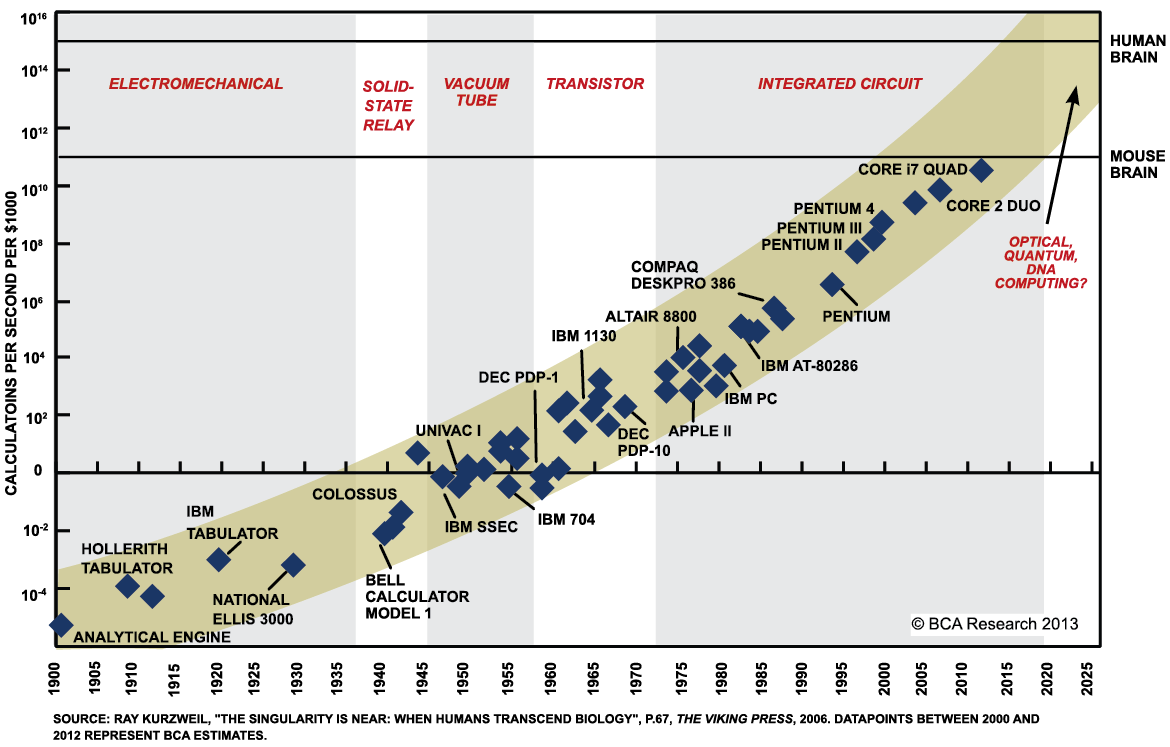
\includegraphics[scale=0.35,center]{MooresLaw}
\\
\\
Elementami niezbędnymi do prawidłowego wykreowania wirtualnego środowiska jest zarówno dedykowane oprogramowanie jak i sprzęt konieczny do przekazywania informacji zwrotnych do użytkownika. Rzeczywistość wirtualna aby zostać możliwie najlepiej zinterpretowana przez ludzki mózg musi jak najbardziej przypominać rzeczywistość w której żyjemy na co dzień. Aby sprostać temu zadaniu najczęściej reprezentuje się ją w postaci trójwymiarowych scen. Tylko ten jeden czynnik powoduje, że do poprawnej symulacji niezbędne są nowoczesne, wysokowydajne procesory i karty graficzne będące w stanie przeprowadzić niezbędne obliczenia.

Jak już wspomniano wirtualna rzeczywistość może znajdować zastosowanie także w nauce w szczególności w dziedzinach w których obiekty zainteresowań są zbyt małe aby być widoczne gołym okiem, takie jak cząsteczki chemiczne lub pojedyncze atomy. Istnieje cały szereg programów przeprowadzających np. symulacje oddziaływań międzycząsteczkowych, zwijania białek (ang. protein folding) czy przeprowadzających obliczenia dynamiki molekularnej (ang. molecular dynamics), a także umożliwiających wizualizację tych symulacji. Stosunkowo niewiele jednak jest rozwiązań dedykowanych wirtualnej rzeczywistości, które mogłyby umożliwić interakcję ze sprzężeniem zwrotnym. 
	
Pracownie Laboratorium Biofizyki na Wydziale Fizyki Uniwersytetu Warszawskiego dysponują sprzętem niezbędnym do realizacji takich zadań. Urządzenie haptyczne Sensable Phantom Omni jest przykładem trójwymiarowego wskaźnika ze zwrotną projekcją momentów sił, którego wykorzystanie otwiera całe spektrum nowych możliwości związanych z realizacją projektów wirtualnej rzeczywiści w biofizyce molekularnej. 
	
Z punktu widzenia osoby zajmującej się szeroko pojętą biofizyką molekularną na szczególną uwagę zasługują związki

\chapter*{Cel i zakres pracy}
\addcontentsline{toc}{chapter}{Cel i zakres pracy}

W ramach niniejszej pracy została przedstawiona implementacja aplikacji narzędziowej z pogranicza biofizyki molekularnej i wirtualnej rzeczywistości. Program służący do interaktywnej (przy aktywnym udziale użytkownika) eksploracji struktur biopolimerów w poszukiwaniu regionów optymalnych ze względu na jakość lokalnego dopasowania strukturalnego wzorca (ang. template) i fragmentów cząsteczki celu (ang. target). Jakość znalezionego dopasowania odwzorowuje zwrotna projekcja momentów sił do urządzenia haptycznego. 
	
Program funkcjonuje w formie wtyczki do pakietu PyMOL, do swojego działania wykorzystuje urządzenia i metody wirtualnej rzeczywistości, a także bioinformatyczne algorytmy pomiaru jakości dopasowania struktur (RMSD), algorytmy wyszukujące optymalne dopasowanie (uliniowienie) strukturalne oraz algorytmy maksymalizujące stopień dopasowania struktur (algorytm Kabsch'a).

Poprawne uruchomienie i korzystanie z prezentowanego programu wymaga zestawienia stanowiska pracy składającego się z elementów przedstawionych na diagramie:
\\
\\
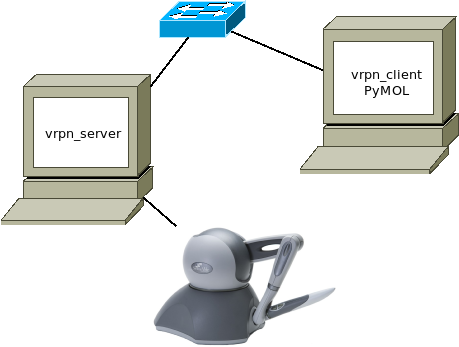
\includegraphics[scale=0.8,center]{stanowisko}
\\
\\
Konfiguracja powyższego stanowiska pracy zostało szczegółowo opisane w dalszej części pracy.

\chapter{Podstawy teoretyczne}
W tym rozdziale zaprezentowano podstawowe twierdzenia oraz teorię leżącą u podstaw niniejszej pracy. Skupiono się na zagadnieniach związanych z przekształceniami geometrycznymi, algorytmami oceny podobieństwa strukturalnego oraz metodami lokalnego dopasowania (uliniawiania) struktur chemicznych.

\section{Metody dopasowania struktur chemicznych}
Celem poszukiwania optymalnych metod dopasowania strukturalnego (ang. structural alignment) jest znalezienie homologii pomiędzy cząsteczkami polimerów lub ich fragmentami jedynie na podstawie kształtu i bez znajomości sekwencji. 

Metody dopasowań strukturalnych pierwotnie odnosiły się do cząsteczek polipeptydów i białek jako podstawowych biopolimerów, szybko jednak ich zastosowanie zostało rozszerzone także na kwasy nukleinowe, w szczególności niekodujący RNA gdyż posiada on ważne funkcje biologiczne (np. enzymatyczne) oraz analogiczne do polipeptydów formy trzeciorzędowe. 

Z uwagi na znacznie wyższą ewolucyjną trwałość struktury przestrzennej w porównaniu do sekwencji (zarówno aminokwasowej jak i nukleotydowej) poszukiwanie dopasowań strukturalnych jest często dużo skuteczniejszą metodą znajdowania związków ewolucyjnych niż klasyczne uliniowienie sekwencji. 

Metody dopasowania możemy podzielić na globalne, których celem jest porównywanie całych struktur trzeciorzędowych oraz lokalne polegające na poszukiwaniu najlepszego dopasowania fragmentu cząsteczki wzorca (np. struktury drugorzędowej) do \textit{podobnego} miejsca w obrębie cząsteczki celu i ewentualna późniejsza ich synteza do dopasowania globalnego.

Kluczowym aspektem tych metod jest efektywna ocena ich jakości. Istnieją zatem dobrze opisane algorytmy służące do szacowania jakości dopasowań strukturalnych. Najczęściej wykorzystywaną do tego celu metryką jest RMSD (ang. root-mean-squared deviation), która zostanie szczegółowo opisana w dalszej części pracy.

Obliczenie dopasowania strukturalnego ponadto implikuje powstanie dopasowania sekwencyjnego pomiędzy przyrównywanymi merami w każdym z łańcuchów. Ocena takiego jednowymiarowego uliniowienia sekwencji również da nam wiedzę o tym jak bliska relacja występuje pomiędzy strukturami.

\subsection{Globalne dopasowanie struktur} 
Z powodu dużej złożoności biopolimerów zostało opracowanych wiele metod upraszczających ich reprezentacje do celów obliczeniowych. Przede wszystkim dąży się do rezygnacji z rozpatrywania lokalizacji wszystkich atomów pochodzących z każdego meru na rzeczy jedynie tych należących do szkieletu (ang. backbone) cząsteczki (np. $\alpha$-węgle aminokwasów czy pentozy kwasów nukleinowych), z pominięciem lub daleko idącym ograniczeniem roli łańcuchów bocznych.

Globalne dopasowanie polega na obliczaniu optymalnego nałożenia na siebie (superpozycji) dwóch struktur. Takie iteracyjne podejście w każdym kolejnym kroku poprzez odpowiednie przesunięcia i obroty struktur dąży do minimalizowania odległości pomiędzy atomami i jest najskuteczniejsze gdy podobieństwo porównywanych struktur jest dostatecznie wysokie aby obliczenia dążyły do optymalnego globalnie rezultatu.

Globalne dopasowanie często jest stosowane do porównywania różnych konformacji tego samego polimeru, na przykład do oceny jakości algorytmów przewidujących strukturę białek. 

\subsection{Lokalne dopasowanie struktur} 
Jak już wspomniano, lokalne dopasowanie polega na przeszukiwaniu części lub całej cząsteczki celu (ang. target) w poszukiwaniu wybranych wcześniej fragmentów struktur zwanych wzorcami (ang. template). Wzorcami mogą być struktury drugorzędowe, miejsca wiążące lub inne dowolnie wybrane fragmenty. Wynikiem przeprowadzonych operacji lokalnego dopasowania jest indeks miejsc do których wzorzec jest \textit{podobny} wraz z ich miarą dopasowania. 

Spośród wielu opracowanych metod realizacji lokalnego dopasowania, warto wspomnieć przede wszystkim o metodzie opartej o deskryptory lokalnej struktury [1], która stanowi podstawę implementacji oprogramowania dostarczającego dane wejściowe do programu będącego przedmiotem niniejszej pracy. 




\section{Przekształcenia geometryczne i ich reprezentacje}
Przekształcenia geometryczne w przestrzeni trójwymiarowej stanowią jedne z elementarnych operacji używanych w niniejszej pracy. Zaliczamy do nich przede wszystkim skalowanie, translacje i rotacje. Wszystkie te operacje można praktycznie zrealizować na kilka sposobów. Ze względu na to, że operują one na milionach punktów w przestrzeni trójwymiarowej (pikseli), optymalne metody numeryczne które je realizują są priorytetem i muszą w maksymalnym stopniu wykorzystywać możliwości oferowane przez komputerowe jednostki obliczeniowe i procesory graficzne. 

Współpraca bibliotek programistycznych pochodzących od różnych dostawców może wymagać konwersji pomiędzy różnymi formatami opisu transformacji. Szczególną uwagę należy zwrócić na konwersję orientacji wskaźnika urządzenia haptycznego z formatu dostarczonego przez bibliotekę VRPN (kwaterniony) na format akceptowany przez PyMOL (oś i kąt obrotu) i odwrotnie - ten aspekt zostanie omówiony w dalszej części pracy.

Z uwagi na konieczność dostosowania transformacji do wykonywania na współczesnych komputerach niezbędne było opracowanie efektywnych obliczeniowo metod numerycznych i reprezentacji tych operacji. Bezpośrednia ich implementacja byłaby dość kłopotliwa gdyż nie dość, że każda z nich musiałaby zostać wykonana oddzielnie, to przede wszystkim nie byłoby to optymalne obliczeniowo rozwiązanie. Do tego celu wybrano ujednolicone narzędzia rozwiązujące powyższe problemy: \textit{elementarne macierze transformacji} i \textit{współrzędne jednorodne}.

\textit{Elementarne macierze transformacji} stanowią łatwy sposób posługiwania się przekształceniami geometrycznymi. Każda z powyższych operacji może zostać opisana jako prosta operacja macierzowa (dodawanie albo mnożenie) modyfikująca zbiór punktów w przestrzeni (który również jest reprezentowany jako macierz). %Macierze przekształceń powstały przede wszystkim z myślą o implementacji na współczesnych komputerach, które bardzo dobrze radzą sobie z obliczeniami macierzowymi. Istnieją dziesiątki rozmaitych bibliotek wspomagających tego typu kalkulacje, ponadto operacje macierzowe można łatwo zrównoleglać i optymalizować.


Często jednak pojawia się sytuacja w której wiele przekształceń geometrycznych jest wykonywanych jednocześnie.Dla przykładu można sobie wyobrazić sytuację w której obiekt należy przesunąć jednocześnie dokonując jego obrotu. Niestety stosowanie samych elementarnych macierzy transformacji uniemożliwia rozwiązanie tej kwestii, dopiero współrzędne jednorodne pozwoliły w pełni wyeliminować ten problem.

\textit{Współrzędne jednorodne} są sposobem reprezentacji punktów przestrzeni $n$-wymiarowej za pomocą układu $n+1$ współrzędnych. Zostały one wprowadzone przez niemieckiego matematyka Augusta Möbiusa w 1827 roku i opisane w jego pracy \textit{Der barycentrische Calcul}. 

Współrzędne jednorodne to narzędzie matematyczne stanowiące pewne udoskonalenie elementarnych macierzy transformacji. Umożliwiają wykonywanie wielu przekształceń jednocześnie i za pomocą jednej operacji macierzowej - mnożenia. Współrzędne jednorodne dają możliwość skumulowania wszystkich transformacji jakie chcemy wykonać na strukturze przestrzennej w jednej odpowiednio zbudowanej macierzy. W dzisiejszych czasach zostały one docenione w wielu dziedzinach nie tylko bezpośrednio związanych z grafiką komputerową ale także w robotyce czy biofizyce.

Poniżej szczegółowo opisane zostały operacje skalowania, translacji oraz rotacji. Dla każdej z tych operacji zostały podane formuły matematyczne, ich reprezentacja za pomocą elementarnych macierzy transformacji oraz współrzędnych jednorodnych. Dodatkowo dla rotacji została przedstawiona reprezentacja kwaternionów.

\iffalse
Ogólną postać przekształceń geometrycznych możemy zdefiniować jako:
$$
\vec{P'}=S*R*\vec{P}+T
$$
\\
gdzie:
\\

$\vec{P}$ jest wektorem $\begin{bmatrix} x \\y \\z \\ \end{bmatrix}$ współrzędnych punktu poddanego transformacjom

$\vec{P'}$ jest wektorem $\begin{bmatrix} x'\\ y'\\ z' \end{bmatrix} $ współrzędnych punktu $\vec{P}$ po dokonanych transformacjach

$S$ reprezentuje operację skalowania

$R$ reprezentuje operację rotacji

$T$ reprezentuje operację translacji
\\
\\
\\
Elementarna rotacja jest rotacją danego punktu wokół jednej z osi układu współrzędnych ($X$, $Y$ lub $Z$).
$$
A=\begin{bmatrix}
s & d & f \\
u & j & k
\end{bmatrix}
$$


$$
T=\begin{bmatrix}
t_x \\
t_y \\
t_z
\end{bmatrix}
$$

Przykładowo mając dany wektor współrzędnych $\vec{X}$ opisujący położenie punktu w przestrzeni trójwymiarowej:

$$
\vec{X}=\begin{bmatrix}
x \\
y \\
z
\end{bmatrix}
$$
możemy zdefiniowac macierz $T(a,b,c)$:

\fi

\subsection{Skalowanie}
Skalowanie to operacja polegająca na mnożeniu współrzędnych obiektu określonego w przestrzeni trójwymiarowej przez współczynniki skalowania. Współczynniki skalowania są dodatnią liczbę rzeczywistą $S$ albo dodatnio określony wektor liczb rzeczywistych $\vec{S}$. W ogólności możemy proporcjonalnie skalować wszystkie składowe wektora współrzędnych niezależnie przez stosowanie wektora o różnych współczynnikach jednak dla potrzeb niniejszej pracy wystarczy, że wykonywane skalowanie będzie operacją mnożenia wektora współrzędnych przez skalar $S$.

Geometryczna intuicja stojąca za operacją skalowania polega na takim przekształceniu współrzędnych danego obiektu, że w zależności od wartości współczynników skalujących może on zostać: 

- niezmieniony, gdy $S=1$

- pomniejszony proporcjonalnie do $S$, gdy $0<S<1$

- powiekszony proporcjonalnie do $S$, gdy $S>1$
\\
\\
Współrzędne punktu $P=(x,y,z)$ po operacji skalowania o wektor współczynników $\vec{S}=[s_x,s_y,s_z]^T$ są równe:

$$
\begin{array}{lr}
x'=x*s_x \\
y'=y*s_y \\
z'=z*s_z
\end{array}
$$

Reprezentacja skalowania za pomocą elementarnych macierzy transformacji polega na stworzeniu takiej macierzy $\hat{S}$, że wartości wektora skalującego $\vec{S}$ zostaną wpisane do niej w następujący sposób:
$$
\hat{S}
=
\begin{bmatrix}
s_x & 0 & 0 \\
0 & s_y & 0 \\
0 & 0 & s_z
\end{bmatrix}
$$
zatem:
$$
\vec{P'}=\hat{S}*\vec{P}
$$

$$
\vec{P'}
=
\begin{bmatrix}
s_x & 0 & 0 \\
0 & s_y & 0 \\
0 & 0 & s_z
\end{bmatrix}
*
\begin{bmatrix} 
x \\ 
y \\ 
z 
\end{bmatrix} 
=
\begin{bmatrix} 
x*s_x \\ 
y*s_y \\ 
z*s_z 
\end{bmatrix}
$$
\\
Aby przedstawić operację skalowania we współrzędnych jednorodnych należy stworzyć nową macierz $\bar{S}$ o rozmiarze o 1 większym, niż macierz elementarna $\hat{S}$ oraz nowy wektor $\dot{\vec{P}}$ o długości o 1 większej niż $\vec{P}$:
$$
\bar{S} 
= 
\begin{bmatrix}
s_x & 0 & 0 & 0 \\
0 & s_y & 0 & 0 \\
0 & 0 & s_z & 0 \\
0 & 0 & 0 & 1
\end{bmatrix}
, 
\dot{\vec{P}}
=
\begin{bmatrix} 
x \\ 
y \\ 
z \\
1
\end{bmatrix} 
$$
zatem:
$$
\dot{\vec{P'}}=\bar{S}*\dot{\vec{P}}
$$
$$
\vec{P_2'} = 
\begin{bmatrix}
s_x & 0 & 0 & 0 \\
0 & s_y & 0 & 0 \\
0 & 0 & s_z & 0 \\
0 & 0 & 0 & 1
\end{bmatrix}
*
\begin{bmatrix} 
x \\ 
y \\ 
z \\
1
\end{bmatrix} 
=
\begin{bmatrix} 
x*s_x \\ 
y*s_y \\ 
z*s_z \\
1
\end{bmatrix}
$$

\subsection{Translacje}
W geometrii euklidesowej translacją nazywamy takie przekształcenie geometryczne, które przenosi każdy punkt określony w przestrzeni o dowolny wektor $\vec{T}$. Translacje (przesunięcia) to kolejna elementarna operacja przekształcenia geometrycznego. W odróżnieniu od skalowania, w przypadku przesunięć w przestrzeni do wektora współrzędnych dodajemy wektor współczynników (liczb rzeczywistych) przesunięcia $\vec{T}$.

Operacja przesunięcia wykorzystana jest w pracy w każdym przypadku zmiany położenia wskaźnika urządzenia haptycznego czy podczas wykonywania operacji superpozycji i dopasowania struktur. Dla punktu $P=(x,y,z)$ operacja przesunięcia o wektor $\vec{T}=[t_x, t_y, t_z]^T$ wygląda następująco:

$$
\begin{array}{lr}
x'=x+t_x \\
y'=y+t_y \\
z'=z+t_z
\end{array}
$$
Z powyższego jasno wynika, że translacje można reprezentować jako operację sumy dwóch wektorów:
$$
\vec{P'}=\vec{P}+\vec{T}
$$
$$
\vec{P'}
=
\begin{bmatrix}
x \\
y \\
z
\end{bmatrix}
+
\begin{bmatrix}
T_x \\
T_y \\
T_z 
\end{bmatrix}
=
\begin{bmatrix}
x+T_x \\
y+T_y \\
z+T_z 
\end{bmatrix}
$$

Reprezentacja przy pomocy współrzędnych jednorodnych ponownie wymaga skonstruowania w odpowiedni sposób macierzy translacji $\bar{T}$ poprzez wpisanie do niej w odpowiednim miejscu wektora translacji $\vec{T}$ oraz wektora współrzędnych $\dot{\vec{P}}$ analogicznie jak w przypadku skalowania:
$$
\bar{T}
=
\begin{bmatrix}
1 & 0 & 0 & T_x \\
0 & 1 & 0 & T_y \\
0 & 0 & 1 & T_z \\
0 & 0 & 0 & 1
\end{bmatrix}
,
\dot{\vec{P}}
=
\begin{bmatrix}
x \\
y \\
z \\
1
\end{bmatrix}
$$
zatem:
$$
\vec{P'}=\bar{T}*\dot{\vec{P}}
$$
$$
\vec{P'}=
\begin{bmatrix}
1 & 0 & 0 & T_x \\
0 & 1 & 0 & T_y \\
0 & 0 & 1 & T_z \\
0 & 0 & 0 & 1
\end{bmatrix}
*
\begin{bmatrix}
x \\
y \\
z \\
1
\end{bmatrix}
=
\begin{bmatrix}
x+T_x \\
y+T_y \\
z+T_z \\
1
\end{bmatrix}
$$
\subsection{Rotacje i kwaterniony}
Trzecią elementarną transformacją jest rotacja. W odróżnieniu od skalowania czy translacji jest operacją bardziej złożoną. Po pierwsze kolejność wykonywania rotacji ma znaczenie ($R_xR_y\neq R_yR_x$), po drugie samych reprezentacji rotacji jest co najmniej kilka. Najpopularniejszym z nich są obroty o zadany kąt wokół jednej z osi układu współrzędnych lub arbitralnej osi obrotu i na tym typie skupiono się w tej pracy.

Współrzędne punktu $P'=(x',y',z')$ będącego wynikiem rotacji punktu $P=(x,y,z)$ wokół poszczególnych osi ($OX$, $OY$, $OZ$) układu współrzędnych o zadany kąt (odpowiednio $\alpha$, $\beta$ i $\gamma$) wyrażają się następująco:
\\
\\
rotacja $P$ wokół osi $OX$:
$$
\begin{array}{lr}
x'=x \\
y'=ycos(\alpha)-zsin(\alpha) \\
z'=ysin(\alpha)+zcos(\alpha)
\end{array}
$$
\\
rotacja $P$ wokół osi $OY$:
$$
\begin{array}{lr}
x'=zsin(\beta)+xcos(\beta) \\
y'=y \\
z'=xcos(\beta)-xcos(\beta)
\end{array}
$$
\\
rotacja $P$ wokół osi $OZ$:
$$
\begin{array}{lr}
x'=xcos(\gamma)-ysin(\gamma) \\
y'=xsin(\gamma)+ycos(\gamma) \\
z'=z
\end{array}
$$
Elementarne macierze przekształceń w tym przypadku wyglądają następująco:
$$
\hat{Rx}(\alpha)
=
\begin{bmatrix}
1 & 0 & 0 \\
0 & cos(\alpha) & -sin(\alpha) \\
0 & sin(\alpha) & cos(\alpha)
\end{bmatrix}
$$
$$
\hat{Ry}(\beta)
=
\begin{bmatrix}
cos(\beta) & 0 & sin(\beta) \\
0 & 1 & 0 \\
-sin(\beta) & 0 & cos(\beta) \\
\end{bmatrix}
$$
$$
\hat{Rz}(\gamma)
=
\begin{bmatrix}
cos(\gamma) & -sin(\gamma) & 0 \\
sin(\gamma) & cos(\gamma) & 0 \\
0 & 0 & 1
\end{bmatrix}
$$
gdzie:

$\hat{Rx}(\alpha)$ obrót wokół osi $OX$ o kąt $\alpha$

$\hat{Ry}(\beta)$ obrót wokół osi $OY$ o kąt $\beta$

$\hat{Rz}(\gamma)$ obrót wokół osi $OZ$ o kąt $\gamma$
\\
\\
Jak wszystkie inne transformacje, rotacje równiez można przedstawić we współrzędnych jednorodnych. Mają one wówczas następującą postać:
$$
\bar{Rx}(\alpha) = 
\begin{bmatrix}
1 & 0 & 0 & 0 \\
0 & cos(\alpha) & -sin(\alpha) & 0 \\
0 & sin(\alpha) & cos(\alpha) & 0 \\
0 & 0 & 0 & 1
\end{bmatrix}
$$
$$
\bar{Ry}(\beta) = 
\begin{bmatrix}
cos(\beta) & 0 & sin(\beta) & 0 \\
0 & 1 & 0 & 0 \\
-sin(\beta) & 0 & cos(\beta) & 0 \\
0 & 0 & 0 & 1
\end{bmatrix}
$$
$$
\bar{Rz}(\gamma) = 
\begin{bmatrix}
cos(\gamma) & -sin(\gamma) & 0 & 0 \\
sin(\gamma) & cos(\gamma) & 0 & 0 \\
0 & 0 & 1 & 0 \\
0 & 0 & 0 & 1
\end{bmatrix}
$$

Poza powyższymi reprezentacjami, rotacje posiadają jeszcze jedną być może najważniejszą z punktu widzenia programisty reprezentację: \textit{kwaterniony}.

Kwaterniony są strukturą algebraiczną stanowiącą rozszerzenie liczb zespolonych. Kwaterniony zostały wprowadzone przez Hamiltona, który poszukiwał wygodnego sposobu opisu mechaniki w przestrzeni trójwymiarowej. 

Kwaternion $q$ to taka czwórka liczb rzeczywistych $x$, $y$, $z$ i $w$ spełniająca równanie:
$$
q=w+xi+yj+zk
$$
gdzie:

$i$, $j$, $k$ - współczynniki urojone takie, że $i^2=j^2=k^2=ijk=-1$

$w$ - część skalarna kwaterniona

$x$, $y$, $z$ - część wektorowa kwaterniona
\\
\\
Kwaterniony mogą stanowic alternatywną wobec współrzędnych jednorodnych lub macierzy transformacji formę opisu rotacji. Dzięki temu możemy z powodzeniem przeprowadzać konwersję pomiędzy nimi a kwaternionami. Dzięki kwaternionom z powodzeniem można przedstawić rotację wokół arbitralnie wybranej osi obrotu. 

Załóżmy, że chcemy stworzyć kwaternion $q$ reprezentujący obrót o kąt $\alpha$ wokół wektora $\vec{v}=[v_x,v_y,v_z]$. Kwaternion taki tworzymy w następujący sposób

$$
\begin{array}{lr}
w=cos(\alpha/2) \\
x=v_x sin(\alpha/2) \\
y=v_y sin(\alpha/2) \\
z=v_z sin(\alpha/2) 
\end{array}
$$

wówczas:
$$
q=cos(\alpha/2)+v_xsin(\alpha/2)i+v_ysin(\alpha/2)j+v_zsin(\alpha/2)k
$$



\section{RMSD}
Efektywna ocena podobieństwa struktur chemicznych jest jednym z kluczowych elementów niniejszej pracy. W bioinformatyce istnieje kilka sposobów oszacowania tej wartości: obok GDT (ang. global distance test) i TM-score (ang. template modeling score) najpopularniejsza i stosunkowo prosta w zastosowaniu jest miara odchylenia średniokwadratowego - RMSD (ang. root-mean-squared deviation). 

Ocena podobieństwa metodą RMSD polega na obliczeniu średniokwadratowej odległości pomiędzy współrzędnymi atomów zawartych w strukturze wzorca (ang. template) i w odpowiednim fragmencie cząsteczki celu (ang. target). W tym przypadku jednostką najczęściej jest \AA (angstrom). Dwie struktury są tym bardziej do siebie podobne im bliższa zeru jest wartość RMSD.

$$
\begin{array}{lr}
RMSD(p,q) = \sqrt{\frac{1}{N}\sum_{i=1}^{N}||p_i-q_i||^{2}} = \\
\\
= \sqrt{\frac{1}{N}\sum_{i=1}^{N}((p_{ix}-q_{ix})^{2}+(p_{iy}-q_{iy})^{2}+(p_{iz}-q_{iz})^{2})}
\end{array}
$$

gdzie:

$p$ - wektor współrzędnych struktury wzorca

$q$ - wektor współrzędnych wybranego regionu w strukturze celu

$N$ - długość wektorów współrzędnych $p$ i $q$
\\
\\
O ile same obliczenia są trywialne, to dobór danych wejściowych do algorytmu RMSD może stanowić poważne wyzwanie. 

W tym przypadku dane pochodzą z zewnętrznej aplikacji, która wykonuje procedurę dopasowania (uliniowienia) struktur wzorca i celu i odnajduje takie regiony, których miara podobieństwa nie przekracza zadanego progu (ang. threshold). Wynikiem takiej procedury są dane mapujące (ang. mapping file) zawierające informację o lokalizacji \textit{regionów podobnych} do struktury wzorca w cząsteczce celu. Takimi regionami mogą być dowolne struktury drugorzędowe (w szczególności alfa-helisy czy beta-harmonijki) lub trzeciorzędowe.

\begin{figure}[H]
\centering
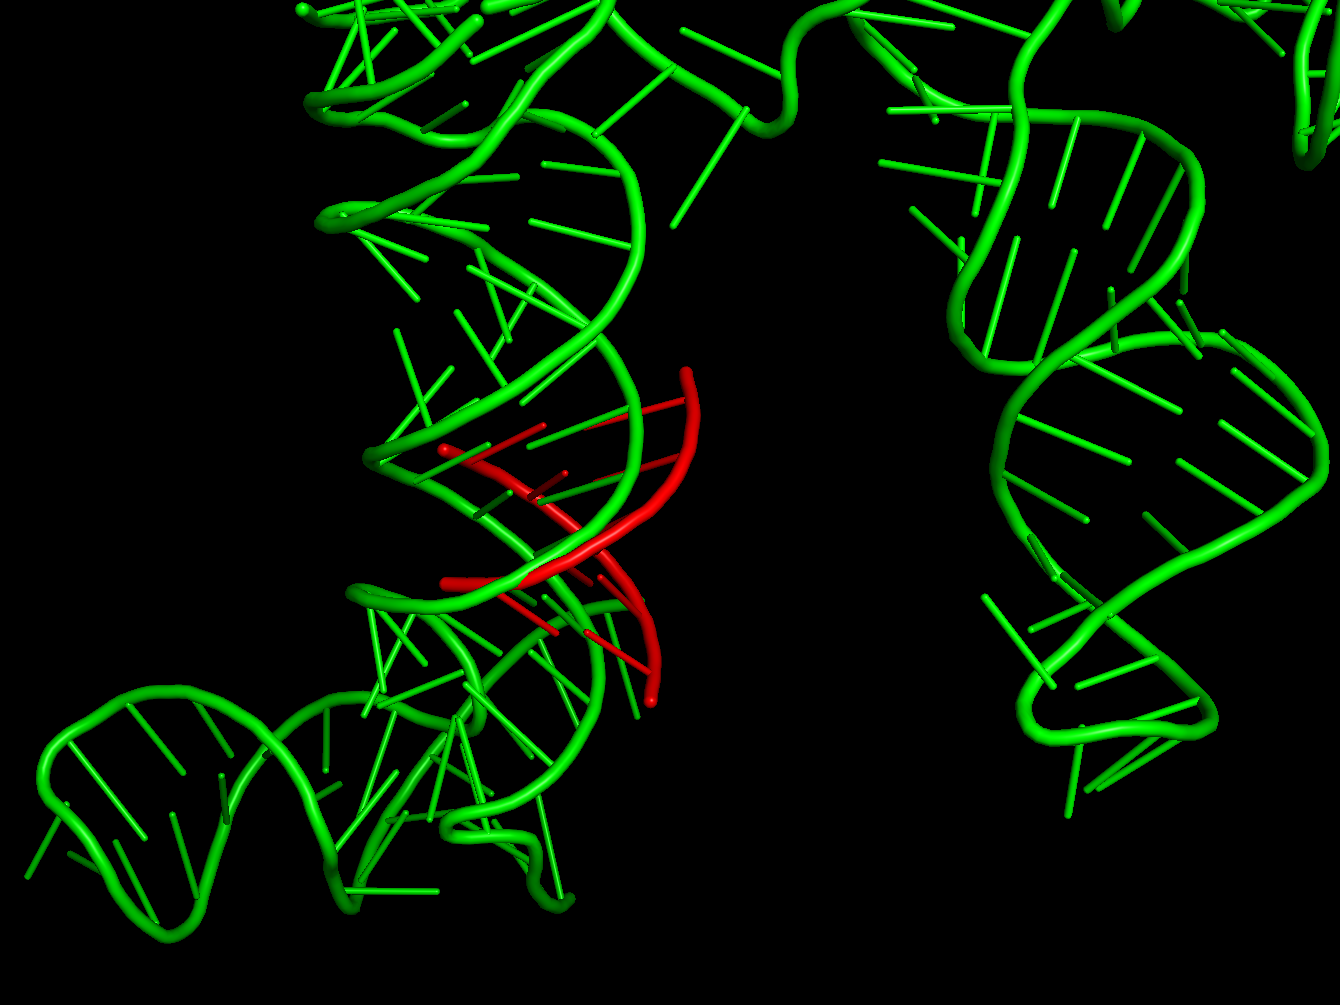
\includegraphics[scale=0.2]{rmsd3}
\caption{Przykładowe dopasowanie struktury wzorca (czerwona) do podobnego regionu struktury celu (zielona), RMSD=3.985}
\end{figure}


\begin{figure}[H]
\centering
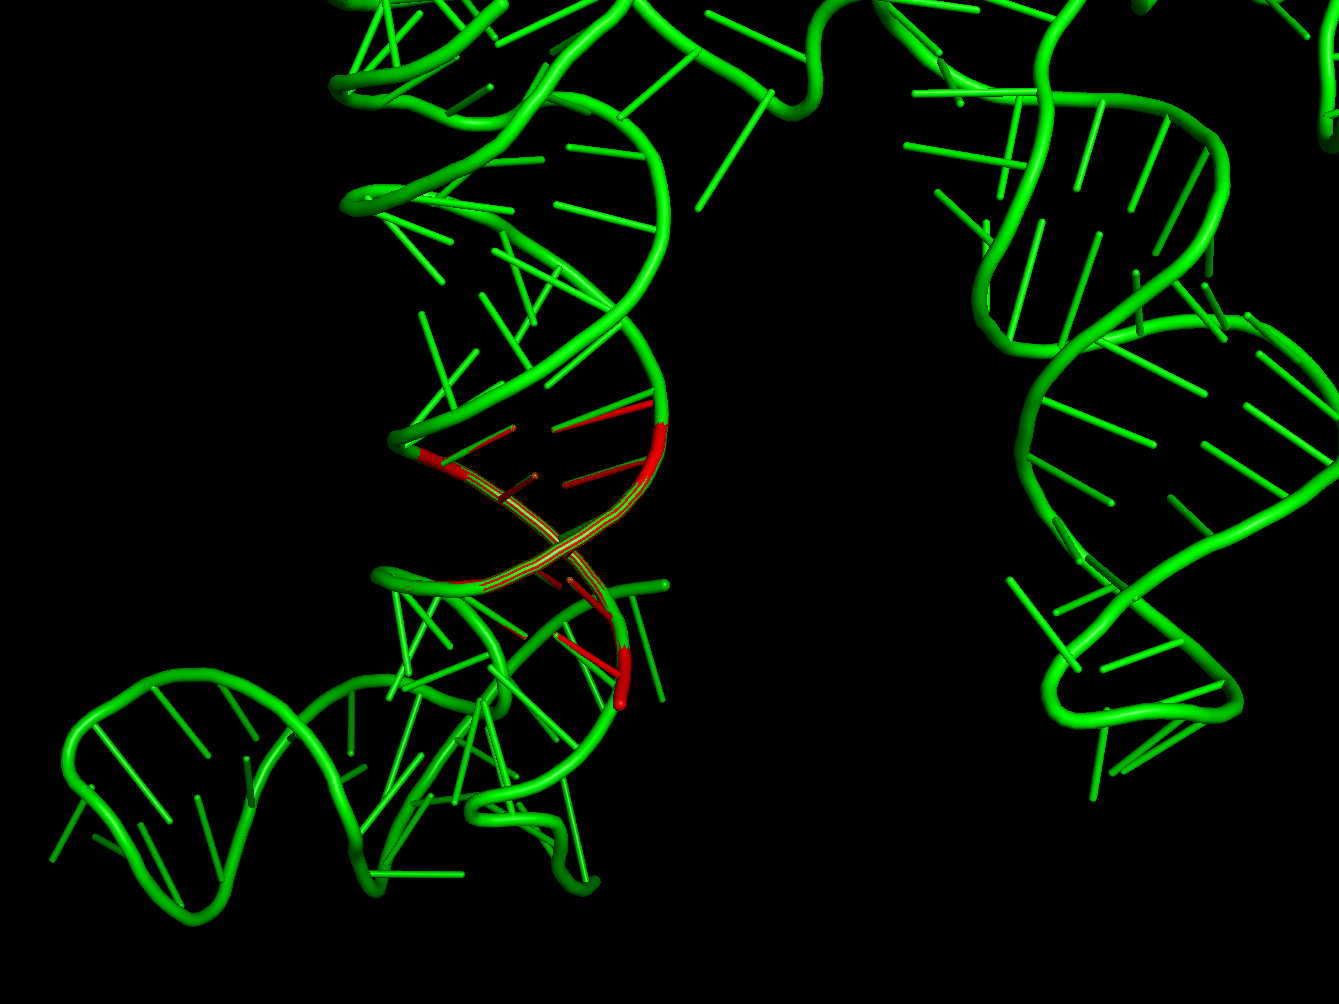
\includegraphics[scale=0.2]{rmsd0}
\caption{Przykładowe dopasowanie struktury wzorca (czerwona) do podobnego regionu struktury celu (zielona), RMSD=0}
\end{figure}

\section{Algorytm Kabsch'a}
RMSD jest jedną podstawowych miar podobieństwa strukturalnego wykorzystywanych w bioinformatyce. Jednym ze znanych sposobów minimalizacji jego wartości jest optymalna translacja i rotacja struktury wzorca nad wybranym regionem struktury celu w taki sposób aby obie struktury zostały jak najlepiej na siebie nałożone. Isteniej kilka metod wyznaczania optymalnych transformacji, jedną z popularniejszych opisał opisał w 1976 roku w swojej pracy [2] Wolfgang Kabsch.

Algorytm startuje z dwoma wektorami współrzędnych $p$ i $q$ o długości $N$. Wektor $p$ stanowi zbiór współrzędnych kartezjańskich struktury wzorca, $q$ - wybranego regionu struktury celu:
$$
p=
\begin{pmatrix}
 x_{p1} & y_{p1} & z_{p1} \\
 x_{p2} & y_{p2} & z_{p2} \\
 \vdots & \vdots & \vdots \\
 x_{pN} & y_{pN} & z_{pN}
\end{pmatrix}
$$
$$
q= 
\begin{pmatrix}
 x_{q1} & y_{q1} & z_{q1} \\
 x_{q2} & y_{q2} & z_{q2} \\
 \vdots & \vdots & \vdots \\
 x_{qN} & y_{qN} & z_{qN}
\end{pmatrix}
$$
\\
Algorytm Kabsch'a składa się z 3 kroków:
\begin{enumerate}
\item \textbf{Translacja} \\
W pierwszym kroku należy dokonać obliczenia centroidów ($Cp$ i $Cq$) obu struktur i dokonać przesunięcia struktury wzorca o wektor $\vec{T}$ rozpięty pomiędzy tymi punktami tak, aby nałożyły się one na siebie. Do obliczenia centroidu można zastosować na przykład równanie na środek geometryczny: 
$$Cp = (Cp_x, Cp_y, Cp_z)$$
gdzie:
$$Cp_x = \frac{1}{N}\sum_{i=1}^{N}{x_{pi}}$$
$$Cp_y = \frac{1}{N}\sum_{i=1}^{N}{y_{pi}}$$
$$Cp_z = \frac{1}{N}\sum_{i=1}^{N}{z_{pi}}$$
oraz
$$Cq = (Cq_x, Cq_y, Cq_z)$$
gdzie:
$$Cq_x = \frac{1}{N}\sum_{i=1}^{N}{x_{qi}}$$
$$Cq_y = \frac{1}{N}\sum_{i=1}^{N}{y_{qi}}$$
$$Cq_z = \frac{1}{N}\sum_{i=1}^{N}{z_{qi}}$$
zatem wektor translacji:
$$ T = |Cp-Cq| =(|Cp_x-Cq_x|,|Cp_y-Cq_y|,|Cp_z-Cq_z|)$$
możemy użyć do wykonania przesunięcia wszystkich punktów w $p$ i $q$:
$$p'=p+T$$
\item \textbf{Macierz kowariancji} \\
Macierz kowariancji $A$ określa zależność liniową między zmiennymi $p$ i $q$. Jej poprawne wyliczenie stanowi podstawę do ustalenia optymalnej macierzy rotacji w kolejnym kroku.
$$ 
A=cov(p,q)
$$
$$
 TODO
$$

\item \textbf{Optymalna macierz rotacji} \\
Optymalna macierz rotacji powstaje z dekompozycji według wartości szczególnych macierzy $A$. SVD (ang. singular value decomposition) to taki rozkład zadanej macierzy na trzy specyficzne macierze $U$, $\Sigma$ oraz $V$, że zachodzi zależność:
$$
A=U \Sigma V^T
$$
$$
 TODO
$$
gdzie:

\quad$U$ i $V$ to macierze ortogonalne (takie, że $U^{-1}=U^{T}$ oraz $V^{-1}=V^{T}$)

\quad$\Sigma$ macierz diagonalna

wówczas optymalną macierz rotacji $R$ uzyskujemy:

$$R=VU^T$$

\end{enumerate}


\section{Pole siłowe}
todo
	
\chapter{Urządzenie haptyczne Sensable Phantom Omni}
Nadrzędnym celem wirtualnej rzeczywistości (ang. virtual reality) jest możliwie wierne odtworzenie świata rzeczywistego w formie programu komputerowego czy multimedialnej prezentacji oraz umożliwienie użytkownikowi wchodzenie w interakcję z tak wykreowanymi scenami. Obecny stan rozwoju techniki pozwala na tworzenie wydajnych urządzeń typu HCI (ang. human computer interface) będących interfejsami pomiędzy światem realnym a wirtualnym. Przykładem takiego urządzenia jest Phantom Omni, opracowane przez firmę Sensable (obecnie Geomagic). 
\\
\\
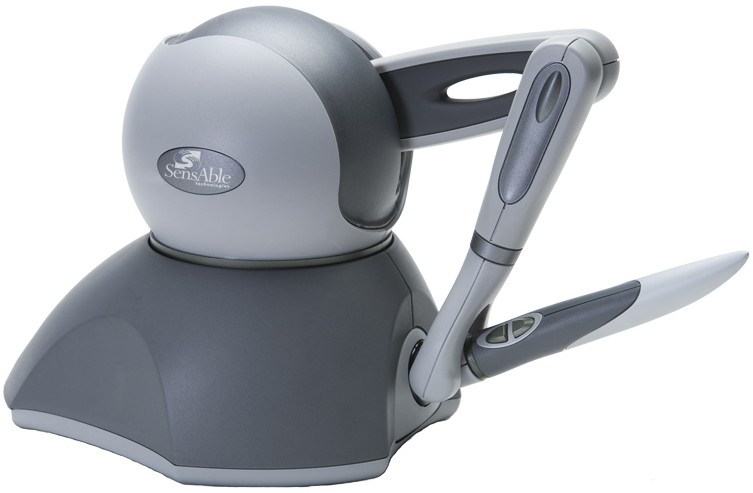
\includegraphics[scale=0.5,center]{Sensable_Phantom_Omni}
\\
\\

Niniejsza praca w dużym stopniu opiera się na wykorzystaniu tych urządzeń do odzworowywania rzeczywistych ruchów ręki użytkownika w świecie wirtualnym. Pracownie Zakładu Biofizyki Wydziału Fizyki Uniwersytetu Warszawskiego są wyposażone w tego typu urządzenia, zostały one udostępnione autorowi celem realizacji niniejszej pracy.

\section{Opis urządzenia}
Urządzenie haptyczne (ang. haptic) Sensable Phantom Omni jest trójwymiarowym wskaźnikiem o 6 stopniach swobody wskazywania pozycji i orientacji z możliwością programowego sterowania zwrotną projekcją momentów sił o trzech stopniach swobody (pozycja wskaźnika). 

Phantom Omni jest wykorzystywany w profesjonalnych rozwiązaniach z zakresu wirtualnej rzeczywistości czy modelowania trójwymiarowego. Umożliwia użytkownikowi wchodzenie w interakcję z cyfrowym światem za pomocą zmysłu dotyku. Wraz z urządzeniem producent dostarcza sterowniki oraz pakiet bibliotek programistycznych OpenHaptics umożliwiających tworzenie oprogramowania w pełni wykorzystującego jego możliwości. 

Specyfikację techniczną urządzenia prezentuje poniższa tabela

\begin{center}
	\begin{tabular}{|l|p{4cm}|}
		\hline Wymiary pola roboczego & szerkość: 160 mm $\newline$ głębokość 70 mm $\newline$ wysokość 120 mm \\
		\hline Rozdzielczość & 450 dpi ($\sim$0.055 mm) \\
		\hline Maksymalny moment obrotowy & 3.3 Nm \\
		\hline Sztywność & oś X: 1.26 N/mm $\newline$ oś Y: 2.31 N/mm $\newline$ oś Z: 1.02 N/mm \\
 		\hline Dane o pozycji i orientacji & osi X, Y i Z $\newline$ kąty $\alpha$, $\beta$ i $\gamma$ $\newline$ (6 stopni swobody)\\
		\hline Zwrotna projekcja sił & osi X, Y i Z $\newline$ (3 stopnie swobody) \\
		\hline Interfejs & IEEE-1394a, Ethernet \\
		\hline
	\end{tabular}
\end{center}

\textbf{TODO:} szczegolowy opis + rysunki
	
\section{Wymagania sprzętowe}

	Urządzenia Sensable Phantom Omni w które wyposażone są Pracownie Biofizyki FUW posiadają dwa rodzaje interfejsów: FireWire (IEEE-1394a) oraz Ethernet. 

Interfejs Ethernet jest powszechnie spotykany w większości komputerów i systemy operacyjne bezproblemowo radzą sobie z jego obsługą. Użycie urządzenia Phantom Omni z interfejsem sieciowym wiąże się jednak z instalacją dedykowanych sterowników oraz pakietu OpenHaptics v3.0, które jak podaje producent są wspierają jedynie systemy do Windows 7 co uniemożliwia korzystanie z nich na nowszych platformach.

FireWire jest standardem łącza szeregowego opracowanym w 1995 roku, który umożliwia szybką transmisję danych. Został on zaprojektowany przede wszystkim do szybkiego przesyłania danych o dużym rozmiarze, zatem jest często wykorzystywany przez producentów sprzętu multimedialnego. Jednak w związku z systematycznym wycofywaniem się (od 2011 roku) producentów sprzętu i oprogramowania ze wspierania interfejsu FireWire, korzystanie z urządzeń w niego wyposażonych rodzi wiele problemów. Użytkownik jest zmuszony do poszukiwania kart rozszerzeń do stacji roboczych mających obsługiwać urządzenia - na dodatek firma SenseAble zaleca korzystanie wyłącznie z kontrolerów IEEE-1394a opartych o chipset firmy NEC lub VIA co jeszcze bardziej utrudnia proces wdrażania.

Powyższe trudności powodują, że sam proces instalacji i uruchomienia urządzenia staje się bardzo kłopotliwy, a często niemożliwy. Stacje robocze korzystające z urządzeń Phantom Omni w Pracowniach Biofizyki FUW działają na systemach operacyjny CentOS w wersji 6.0, który pozwalał na stosunkowo stabilne działanie urządzenia. Wraz ze sterownikami i pakietem OpenHaptics w pracowniach uruchomiony jest framework VRPN (Virtual Reality Perfipherial Network), który został opisany w dalszej części pracy.

Proces instalacji i konfiguracji urządzenia SensAble Phantom Omni nie był przedmiotem niniejszej pracy.

\section{OpenHaptics Toolkit v3.0}

OpenHaptics Toolkit v3.0 jest bogatym pakietem oprogramowania dostarczanego przez producenta urządzenia. Zawiera on zestaw sterowników, bibliotek, narzędzi i przykładowych kodów źródłowych ułatwiających programiście wrożenie rozwiązań haptycznych w dowolnym programie komputerowym. Biblioteki programistyczne dają dostęp do szerokiego zakresu niskopoziomowych funkcji urządzenia Phantom Omni tworząc przyjazną dla programisty abstrakcję. 
\\
\\
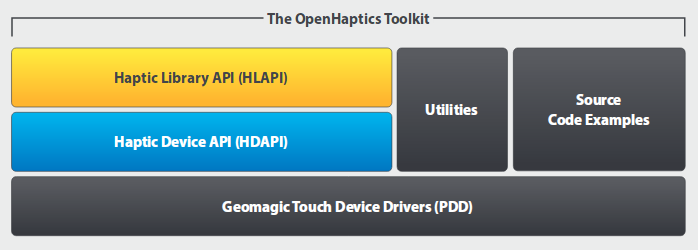
\includegraphics[scale=0.5,center]{openhaptics}
\\
\\

\subsection{Phantom Device Drivers}
Phantom Device Drivers (PDD) to zestaw sterowników do różnych urządzeń haptycznych oferowanych przez producenta.



\subsection{Haptic Device API}
- Haptic Device API (HDAPI) – niskopoziomowe API umożliwiające bezpośredni dostęp do funkcji sterujących projekcją sił i pobieraniem danych o pozycji i orientacji wskaźnika


\subsection{Haptic Library Api}
- Haptic Library API (HLAPI) – wysokopoziomowe API zaprojektowane głównie pod kątem zgodności składniowej z OpenGL API



\section{Przykłady wykorzystania}
tu beda jakies rzeczy...
sdf
sdf
sdf
s
sdf
s

sd

sdf
sdf


sdf

sdf

sdf

sd

sdf

sdf

sfd

sdf

sdf

sdf

sdf

sdf

sdf

sd

sdf




\chapter{Biblioteka VRPN}
ll

\section{Opis pakietu}
opisik

\section{Dostosowanie VRPN do wymagań niniejszej pracy}
opis

\section{Kompilacja i uruchomienie}
kompilacja i uruchomienie

\chapter{Pakiet PyMOL}
PyMOL jest oprogramowaniem służącym głównie do wizualizacji struktur chemicznych oraz przeprowadzania na nich prostych obliczeń. Jego historia sięga roku 2000, kiedy to Warren Lyford DeLano zainicjował powstanie projektu. Przez lata intensywnych prac nad rozwojem program stał się standardowym narzędziem wykorzystywanym przez wiele wiodących ośrodków naukowo badawczych. Obecnie nad jego rozwojem czuwa firma \textit{Schrödinger, Inc}.

\section{Opis Oprogramowania}
opisik

\section{Rozszerzanie funkcjonalności pakietu PyMOL}
Funkcjonalność pakiet PyMOL może być w łatwy sposób rozszerzalna poprzez wbudowany system obsługi wtyczek (ang. plugin) tworzonych w języku Python. Programista ma dostęp do rozbudowanego API (ang. application programming interface) zawierającego szeroki wachlarz funkcji umożliwiających prowadzenie różnych obliczeń na załadowanych strukturach. Ponadto programista tworząc wtyczki może z powodzeniem korzystać z biblioteki standardowej języka Python oraz dowolnych bibliotek zewnętrznych autorów.

Podczas tworzenia oprogramowania będącego przedmiotem niniejszej pracy korzystano zarówno z API wbudowanego w PyMOL jak również z zewnętrznych bibliotek takich jak VRPN do obsługi urządzenia haptycznego.

Tworzenie wtyczek polega na zdefiniowaniu funkcji \textbf{\_\_init\_\_(self)}, która podczas uruchamiania programu PyMOL tworzy nową pozycję w menu. Jednym z jej parametrów jest referencję do głównej funkcji programu rozszerzającego (wtyczki). Taką funkcję należy zdefiniować w osobnym pliku z rozszerzeniem \textit{.py}.

\section{Uruchamianie wtyczek w ramach środowiska PyMOL}

\chapter{Opis stanowiska laboratoryjnego}


\iffalse
\chapter{Podstawowe pojęcia}\label{r:pojecia}

Pojęciem pierwotnym blabalii fetorycznej jest \emph{blaba}.
Blabaliści nie podają jego definicji, mówiąc za Ciach-Pfe t-\=am
K\^un (fooistyczny mędrzec, XIX w. p.n.e.):
\begin{quote}
  Blaba, który jest blaba, nie jest prawdziwym blaba.

\raggedleft\slshape tłum. z~chińskiego Robert Blarbarucki
\end{quote}

\section{Definicje}

Oto dwie definicje wprowadzające podstawowe pojęcia blabalii
fetorycznej:

\begin{defi}\label{skupienie}
  Silny, zwarty i gotowy fetor bazowy nazwiemy \emph{skupieniem}.
\end{defi}

\begin{defi}\label{fetor}
  \emph{Fetorem} nazwiemy skupienie blaba spełniające następujący
  \emph{aksjomat reperkusatywności}:
  $$\forall \mathcal{X}\in Z(t)\ \exists
  \pi\subseteq\oint_{\Omega^2}\kappa\leftrightarrow 42$$
\end{defi}


\section{Blabalizator różnicowy}

Teoretycy blabalii (zob. np. pracę~\cite{grglo}) zadowalają się
niekonstruktywnym opisem natury fetorów.

Podstawowym narzędziem blabalii empirycznej jest blabalizator
różnicowy.  Przyrząd ten pozwala w~sposób przybliżony uzyskać
współczynniki rozkładu Głombaskiego dla fetorów bazowych
i~harmonicznych.  Praktyczne znaczenie tego procesu jest oczywiste:
korzystając z~reperkusatywności pozwala on przejść do przestrzeni
$\Lambda^{\nabla}$, a~tym samym znaleźć retroizotonalne współczynniki
semi-quasi-celibatu dla klatek Rozkoszy (zob.~\cite{JR}).

Klasyczne algorytmy dla blabalizatora różnicowego wykorzystują:
\begin{enumerate}
\item dualizm falowo-korpuskularny, a w szczególności
  \begin{enumerate}
  \item korpuskularną naturę fetorów,
  \item falową naturę blaba,
  \item falowo-korpuskularną naturę gryzmołów;
  \end{enumerate}
\item postępującą gryzmolizację poszczególnych dziedzin nauki, w
  szczególności badań systemowych i rozcieńczonych;
\item dynamizm fazowy stetryczenia parajonizacyjnego;
\item wreszcie tradycyjne opozycje:
  \begin{itemize}
  \item duch --- bakteria,
  \item mieć --- chcieć,
  \item myśl --- owsianka,
  \item parafina --- durszlak\footnote{Więcej o tym przypadku --- patrz
      prace Gryzybór-Głombaskiego i innych teoretyków nurtu
      teoretyczno-praktycznego badań w~Instytucie Podstawowych
      Problemów Blabalii w~Fifie.},
  \item logos --- termos\footnote{Szpotański}
  \end{itemize}
  z właściwym im przedziwym dynamizmem.
\end{enumerate}

\begin{figure}[tp]
  \centering
  \framebox{\vbox to 4cm{\vfil\hbox to
      7cm{\hfil\tiny.\hfil}\vfil}}
  \caption{Artystyczna wizja blaba w~obrazie węgierskiego artysty
    Josipa~A. Rozkoszy pt.~,,Blaba''}
\end{figure}

\chapter{Wcześniejsze implementacje blabalizatora
  różnicowego}\label{r:losers}

\section{Podejście wprost}

Najprostszym sposobem wykonania blabalizy jest siłowe przeszukanie
całej przestrzeni rozwiązań.  Jednak, jak łatwo wyliczyć, rozmiar
przestrzeni rozwiązań rośnie wykładniczo z~liczbą fetorów bazowych.
Tak więc przegląd wszystkich rozwiązań sprawdza się jedynie dla bardzo
prostych przestrzeni lamblialnych.  Oznacza to, że taka metoda ma
niewielkie znaczenie praktyczne --- w~typowym przypadku z~życia trzeba
rozważać przestrzenie lamblialne wymiaru rzędu 1000.

W~literaturze można znaleźć kilka prób opracowania heurystyk dla
problemu blabalizy (por. \cite{heu}).  Korzystając z~heurystyk daje
się z~pewnym trudem dokonać blabalizy w~przestrzeni o~np.~500 fetorach
bazowych.  Należy jednak pamiętać, że heurystyka nie daje gwarancji
znalezienia najlepszego rozwiązania.  Fifak w~pracy~\cite{ff-sr}
podaje, jak dla dowolnie zadanej funkcji oceniającej skonstruować
dane, dla których rozwiązanie wygenerowane przez algorytm heurystyczny
jest dowolnie odległe od rzeczywistego.

\section{Metody wykorzystujące teorię Głombaskiego}

Teoria Głombaskiego (zob.~\cite{grglo}) dostarcza eleganckiego
narzędzia opisu przejścia do przestrzeni $\Lambda^{\nabla}$.
Wystarczy mianowicie przedstawić fetory bazowe wyjściowej przestrzeni
lamblialnej w~nieskończonej bazie tak zwanych wyższych aromatów.
(Formalną definicję tego pojęcia przedstawię w~rozdziale poświęconym
teorii Fifaka).  Podstawową cechą wyższych aromatów jest ulotność.  To
zaś oznacza, że odpowiednio dobierając współczynniki przejścia do
przestrzeni wyższych aromatów można zagwarantować dowolną z~góry
zadaną dokładność przybliżonego rozwiązania problemu blabalizy.

Oczywiście ze względu na nieskończony wymiar przestrzeni wyższych
aromatów koszt poszukiwania współczynników blabalizy jest liniowy ze
względu na wymiar wyjściowej przestrzeni lamblialnej.

\section{Metody wykorzystujące własności fetorów $\sigma$}

Najchętniej wykorzystywaną przestrzenią wyższych aromatów jest
przestrzeń fetorów~$\sigma$.  Fetory $\sigma$ dają szczególnie prostą
bazę podprzestrzeni widłowej.  Wiąże się to z~faktem, że w~tym przypadku
fetory harmoniczne wyższych rzędów są pomijalne (rzędu $2^{-t^3}$,
gdzie $t$ jest wymiarem wyjściowej przestrzeni lamblialnej).

Niestety z~fetorami $\sigma$ wiąże się też przykre ograniczenie: można
wykazać (zob.~\cite[s. 374]{ff-sr}), że dla dowolnie dobranej bazy
w~podprzestrzeni widłowej istnieje ograniczenie dolne w~metryce sierpa
na odległość rzutu dokładnego rozwiązania problemu blabalizy na
podprzestrzeń widłową.  Ponieważ rzut ten stanowi najlepsze
przybliżone rozwiązanie, jakie można osiągnąć nie naruszając aksjomatu
reperkusatywności, więc istnieje pewien nieprzekraczalny próg
dokładności dla blabalizy wykonanej przez przejście do przestrzeni
fetorów $\sigma$.  Wartość retroinicjalną tego progu nazywa się
\textit{reziduum blabicznym}.

\chapter{Teoria fetorów $\sigma$-$\rho$}\label{r:fifak}

Głównym odkryciem Fifaka jest, że fetor suprakowariantny może
gryzmolizować dowolny ideał w~podprzestrzeni widłowej przestrzeni
lamblialnej funkcji Rozkoszy.

Udowodnienie tego faktu wymagało wykorzystania twierdzeń pochodzących
z~kilku niezależnych teorii matematycznych (zob. na przykład:
\cite{russell,spyrpt,JR,beaman,hopp,srinis}).  Jednym z~filarów
dowodu jest teoria odwzorowań owalnych Leukocyta (zob.~\cite{leuk}).

Znaczenie twierdzenia Fifaka dla problemu blabalizy polega na tym, że
znając retroizotonalne współczynniki dla klatek Rozkoszy można
przeprowadzić fetory bazowe na dwie nieskończone bazy fetorów $\sigma$
w~przestrzeni $K_7$ i~fetorów $\rho$ w~odpowiedniej
quasi-quasi-przestrzeni równoległej (zob.~\cite{hopp}).  Zasadnicza
różnica w~stosunku do innych metod blabalizy polega na tym, że
przedstawienie to jest dokładne.

\chapter{Dokumentacja użytkowa i~opis implementacji}\label{r:impl}

Program przygotowany dla systemu operacyjnego M\$ Windows uruchamia
się energicznym dwumlaskiem na jego ikonce w~folderze
\verb+\\FIDO\FOO\BLABA+.  Następnie kolistym ruchem ręki należy
naprowadzić kursor na menu \texttt{Blabaliza} i~uaktywnić pozycję
\texttt{Otwórz plik}.  Po wybraniu pliku i~zatwierdzeniu wyboru
przyciskiem \texttt{OK} rozpocznie się proces blabalizy.  Wyniki
zostaną zapisane w~pliku o~nazwie \texttt{99-1a.tx.43} w~bieżącym
folderze.

\chapter{Podsumowanie}

W~pracy przedstawiono pierwszą efektywną implementację blabalizatora
różnicowego.  Umiejętność wykonania blabalizy numerycznej dla danych
,,z życia'' stanowi dla blabalii fetorycznej podobny przełom, jak dla
innych dziedzin wiedzy stanowiło ogłoszenie teorii Mikołaja Kopernika
i~Gryzybór Głombaskiego.  Z~pewnością w~rozpocznynającym się XXI wieku
będziemy obserwować rozkwit blabalii fetorycznej.

Trudno przewidzieć wszystkie nowe możliwości, ale te co bardziej
oczywiste można wskazać już teraz.  Są to:
\begin{itemize}
\item degryzmolizacja wieńców telecentrycznych,
\item realizacja zimnej reakcji lambliarnej,
\item loty celulityczne,
\item dokładne obliczenie wieku Wszechświata.
\end{itemize}

\section{Perspektywy wykorzystania w~przemyśle}

Ze względu na znaczenie strategiczne wyników pracy ten punkt uległ
utajnieniu.

\appendix

\chapter{Główna pętla programu zapisana w~języku T\=oFoo}

\begin{verbatim}
[[foo]{,}[[a3,(([(,),{[[]]}]),
  [1; [{,13},[[[11],11],231]]].
  [13;[!xz]].
  [42;[{,x},[[2],{'a'},14]]].
  [br;[XQ*10]].
 ), 2q, for, [1,]2, [..].[7]{x}],[(((,[[1{{123,},},;.112]],
        else 42;
   . 'b'.. '9', [[13141],{13414}], 11),
 [1; [[134,sigma],22]].
 [2; [[rho,-],11]].
 )[14].
 ), {1234}],]. [map [cc], 1, 22]. [rho x 1]. {22; [22]},
       dd.
 [11; sigma].
        ss.4.c.q.42.b.ll.ls.chmod.aux.rm.foo;
 [112.34; rho];
        001110101010101010101010101010101111101001@
 [22%f4].
 cq. rep. else 7;
 ]. hlt
\end{verbatim}

\chapter{Przykładowe dane wejściowe algorytmu}

\begin{center}
  \begin{tabular}{rrr}
    $\alpha$ & $\beta$ & $\gamma_7$ \\
    901384 & 13784 & 1341\\
    68746546 & 13498& 09165\\
    918324719& 1789 & 1310 \\
    9089 & 91032874& 1873 \\
    1 & 9187 & 19032874193 \\
    90143 & 01938 & 0193284 \\
    309132 & $-1349$ & $-149089088$ \\
    0202122 & 1234132 & 918324098 \\
    11234 & $-109234$ & 1934 \\
  \end{tabular}
\end{center}

\chapter{Przykładowe wyniki blabalizy
    (ze~współczynnikami~$\sigma$-$\rho$)}

\begin{center}
  \begin{tabular}{lrrrr}
    & Współczynniki \\
    & Głombaskiego & $\rho$ & $\sigma$ & $\sigma$-$\rho$\\
    $\gamma_{0}$ & 1,331 & 2,01 & 13,42 & 0,01 \\
    $\gamma_{1}$ & 1,331 & 113,01 & 13,42 & 0,01 \\
    $\gamma_{2}$ & 1,332 & 0,01 & 13,42 & 0,01 \\
    $\gamma_{3}$ & 1,331 & 51,01 & 13,42 & 0,01 \\
    $\gamma_{4}$ & 1,332 & 3165,01 & 13,42 & 0,01 \\
    $\gamma_{5}$ & 1,331 & 1,01 & 13,42 & 0,01 \\
    $\gamma_{6}$ & 1,330 & 0,01 & 13,42 & 0,01 \\
    $\gamma_{7}$ & 1,331 & 16435,01 & 13,42 & 0,01 \\
    $\gamma_{8}$ & 1,332 & 865336,01 & 13,42 & 0,01 \\
    $\gamma_{9}$ & 1,331 & 34,01 & 13,42 & 0,01 \\
    $\gamma_{10}$ & 1,332 & 7891432,01 & 13,42 & 0,01 \\
    $\gamma_{11}$ & 1,331 & 8913,01 & 13,42 & 0,01 \\
    $\gamma_{12}$ & 1,331 & 13,01 & 13,42 & 0,01 \\
    $\gamma_{13}$ & 1,334 & 789,01 & 13,42 & 0,01 \\
    $\gamma_{14}$ & 1,331 & 4897453,01 & 13,42 & 0,01 \\
    $\gamma_{15}$ & 1,329 & 783591,01 & 13,42 & 0,01 \\
  \end{tabular}
\end{center}

\fi

\begin{thebibliography}{99}
\addcontentsline{toc}{chapter}{Bibliografia}

\bibitem[Bea65]{beaman} Juliusz Beaman, \textit{Morbidity of the Jolly
    function}, Mathematica Absurdica, 117 (1965) 338--9.

\bibitem[Blar16]{eb1} Elizjusz Blarbarucki, \textit{O pewnych
    aspektach pewnych aspektów}, Astrolog Polski, Zeszyt 16, Warszawa
  1916.

\bibitem[Fif00]{ffgg} Filigran Fifak, Gizbert Gryzogrzechotalski,
  \textit{O blabalii fetorycznej}, Materiały Konferencji Euroblabal
  2000.

\bibitem[Fif01]{ff-sr} Filigran Fifak, \textit{O fetorach
    $\sigma$-$\rho$}, Acta Fetorica, 2001.

\bibitem[Głomb04]{grglo} Gryzybór Głombaski, \textit{Parazytonikacja
    blabiczna fetorów --- nowa teoria wszystkiego}, Warszawa 1904.

\bibitem[Hopp96]{hopp} Claude Hopper, \textit{On some $\Pi$-hedral
    surfaces in quasi-quasi space}, Omnius University Press, 1996.

\bibitem[Leuk00]{leuk} Lechoslav Leukocyt, \textit{Oval mappings ab ovo},
  Materiały Białostockiej Konferencji Hodowców Drobiu, 2000.

\bibitem[Rozk93]{JR} Josip A.~Rozkosza, \textit{O pewnych własnościach
    pewnych funkcji}, Północnopomorski Dziennik Matematyczny 63491
  (1993).

\bibitem[Spy59]{spyrpt} Mrowclaw Spyrpt, \textit{A matrix is a matrix
    is a matrix}, Mat. Zburp., 91 (1959) 28--35.

\bibitem[Sri64]{srinis} Rajagopalachari Sriniswamiramanathan,
  \textit{Some expansions on the Flausgloten Theorem on locally
    congested lutches}, J. Math.  Soc., North Bombay, 13 (1964) 72--6.

\bibitem[Whi25]{russell} Alfred N. Whitehead, Bertrand Russell,
  \textit{Principia Mathematica}, Cambridge University Press, 1925.

\bibitem[Zen69]{heu} Zenon Zenon, \textit{Użyteczne heurystyki
    w~blabalizie}, Młody Technik, nr~11, 1969.

\end{thebibliography}

\chapter*{Kod źródłowy programu}

\begin{lstlisting}
# -*- coding: utf-8 -*-

"""
    This program was created in 2015-16 by Pawel Tomaszewski
    In cooperation with Biophysics Laboratory of Warsaw University
"""

import os
import sys
sys.path.append("/home/crooveck/workspace/LICENCJAT/python_vrpn")
sys.path.append(".")
from transformations import *
from Tkinter import *
from tkFileDialog import *
#from ttk import *
from pymol import *
from pymol.cgo import *
from time import *
import vrpn_Tracker
import vrpn_Button
import vrpn_ForceDevice
from math import *

"""
    Mainloop running flag. This indicates if threads and mainloops are running.
"""
IS_RUNNING = False
AUTO_ZOOMING = False
AUTO_DOCK=False
REGION_COLOR=False

"""
    Global variables for translations. 
    trackerX,trackerY,trackerZ - Phantom native coordinates
    x,y,z - Pymol coordinates
    scale - ratio between PYMOL and PHANTOM coordinate
"""
trackerX = trackerY = trackerZ = 0
x = y = z = 0 
scale=750
templeCOM=(0,0,0)

"""
    Global variables for rotations
    previous_orientation stores a quaternion that represent previous orientation
"""
previous_orientation=0

"""
    center of mass of a loaded molecule
"""
molecule_com=[0,0,0]    
mapping=[]
regions={}

currentWindow=0
mappingFile=0
phantomIp=0
structureFile=0
templateFile=0
# zmienne do wyswietlania danych w UI
regionId=regionX=regionY=regionZ=regionTemplateDistance=rmsdEntry=0

def simple_com(region_coordinates):
    # pobiera jako parametr liste z krotkami ze wspolrzednymi i zwraca srodek masy
    x, y, z = 0,0,0
    size = len(region_coordinates)
    
    for coordinate in region_coordinates:
        x += coordinate[0]
        y += coordinate[1]
        z += coordinate[2]
        
    return (x/size, y/size, z/size)

def tracker_handler(u, tracker):
    global trackerX, trackerY, trackerZ
    trackerX = tracker[1]
    trackerY = tracker[2]
    trackerZ = tracker[3]
    
#   TRANSLACJE:
    x0 = trackerX*scale
    y0 = trackerY*scale
    z0 = trackerZ*scale
#   funkcja dokonujaca przeksztalcenia - transjacji
    global x, y, z
    cmd.translate(vector=[(x0-x), (y0-y), (z0-z)], object="template", camera=1)
    x = x0
    y = y0
    z = z0
    
#   ROTACJE 
    global previous_orientation
    # bierzacy stan - orientacja
    orientation=(tracker[7],tracker[4],tracker[5],tracker[6])   # inny format kwaterniona do transformations.py niz dostaje z VRPN
    # przy pierwszym uruchomieniu 
    # gdy nie ma poprzedniej orientacji 
    if(previous_orientation == 0):
        previous_orientation=orientation

    rotation_quaternion=quaternion_multiply(quaternion_inverse(previous_orientation),orientation)
    previous_orientation=orientation
    
    rotation_matrix = quaternion_matrix(rotation_quaternion) # Return homogeneous rotation matrix from quaternion.
    (rotation_angle,rotation_axis,point) = rotation_from_matrix(rotation_matrix)


    cmd.rotate(axis=[rotation_axis[0],rotation_axis[1],rotation_axis[2]], 
            angle=(rotation_angle*180/math.pi), origin=[templeCOM[0],templeCOM[1],templeCOM[2]], object="template", camera=1)


#    cmd.rotate(axis=[rotation_axis[0],rotation_axis[1],rotation_axis[2]], 
#            angle=(rotation_angle*180/math.pi), origin=[x,y,z], object="template", camera=1)


def button_handler(u, button):
    # button[0] - numer przycisku (0-gorny,1-dolny)
    # button[1] - status przycisku (0-puszczony,1-wcisniety)
    
    global AUTO_ZOOMING, AUTO_DOCK
    if(button[0]==0 and button[1]==0):
        AUTO_ZOOMING = False
    elif(button[0]==0 and button[1]==1):
        AUTO_ZOOMING = True
        
    if(button[0]==1 and button[1]==0):
        print "<< Puszczony przycisk 2 >>"
        
    elif(button[0]==1 and button[1]==1):
        print "ALIGN: ",cmd.align("template","region")
        com=cmd.centerofmass("template")
        cmd.translate(object="template",vector=[x-com[0],y-com[1],z-com[2]],camera=0)
#        print "COM TEMPLATE:", cmd.centerofmass("template"), x, y, z
        
def force_handler(u, force):
#    print "force",force
    abc='test'
    
def draw_template_structure(template_pdb_file):
    cmd.load(template_pdb_file,"template")
    cmd.hide("lines","template")
    cmd.show("cartoon","template")
    cmd.color("green","template")
    
    template_com=cmd.centerofmass("template")
    # centruje wskaxnik (przenosze go do zera)
    cmd.translate(vector=[-template_com[0], -template_com[1], -template_com[2]], object="template", camera=0)
    
def draw_xyz_axes(x0, y0, z0):
    w = 0.5 # cylinder width
    l = 10 # cylinder length
    h = 2 # cone hight
    d = w * 1.618 # cone base diameter
    
    axes = [
        CYLINDER, x0, y0, z0, l, 0.0, 0.0, w, 1.0, 0.0, 0.0, 1.0, 0.0, 0.0,
        CYLINDER, x0, y0, z0, 0.0, l, 0.0, w, 0.0, 1.0, 0.0, 0.0, 1.0, 0.0,
        CYLINDER, x0, y0, z0, 0.0, 0.0, l, w, 0.0, 0.0, 1.0, 0.0, 0.0, 1.0,
        CONE, l, 0.0, 0.0, (h+l), 0.0, 0.0, d, 0.0, 1.0, 0.0, 0.0, 1.0, 0.0, 0.0, 1.0, 1.0,
        CONE, 0.0, l, 0.0, 0.0, (h+l), 0.0, d, 0.0, 0.0, 1.0, 0.0, 0.0, 1.0, 0.0, 1.0, 1.0,
        CONE, 0.0, 0.0, l, 0.0, 0.0, (h+l), d, 0.0, 0.0, 0.0, 1.0, 0.0, 0.0, 1.0, 1.0, 1.0]

    cmd.load_cgo(axes, "axes")
    
def draw_molecule(molecule_pdb_file):
    # laduje czasteczke
    cmd.load(molecule_pdb_file,"molecule")
    cmd.hide("lines","molecule")
    cmd.show("cartoon","molecule")
    cmd.color("red","molecule")
    
    # licze jej centrum masy
    global molecule_com
    molecule_com=cmd.centerofmass("molecule")
    # przesuwam ja na srodek ekranu, srodek ciezkosci na (x,y,z)=(0,0,0)
    cmd.translate(vector=[-molecule_com[0], -molecule_com[1], -molecule_com[2]], object="molecule", camera=0)
    
    # pobieram liste pozycji 3D atomow w czasteczce
    stored.pos = []                                                                                                                
    cmd.iterate_state(1, "molecule", "stored.pos.append((x,y,z,elem,chain,resi))")
    

"""
    Funkcja oblicza wartość RMSD.
    Na wejściu dostaje wektor (listę) współrzędnych struktury wzorcowej oraz
    wektor/listę (tego samego rozmiaru) współrzędnych regionu optymalnego dopasowania,
    zwraca wartość RMDS
"""
def rmsd_compute():
    
    
    
    return 0.0

def load_mapping_file(mapping_file):
    file=open(mapping_file,"r")
    
    global mapping
    mapping=[]

    for line in file:
        mapping_symbol=line.split()[0]
        chain=line.split()[1][0]
        resi=line.split()[1][1:]
        mapping.append([mapping_symbol,chain,resi,0])
    file.close()
    
    # na ostatnie pole w mapping wstawiam COM obliczony dla kazdego nukleotydu
    for nucleotyde in mapping:  # iteruje po wszystkich liniach z pliku mapujacego
        # pobieram atomy nalezace do poszczegolnych nukleotydow
        nucl_coords = [[atom[0],atom[1],atom[2]] for atom in stored.pos if (atom[5]==nucleotyde[2])]
        nucleotyde[3]=simple_com(nucl_coords) # srodek masy dla nukleotydu
        
    print "SKONCZYLEM LADOWANIE MAPOWANIA"
    
def calculate_regions_com():
    # zliczam ilosc nukleotydow w helisie wzorcowej
    # UWAGA: tutaj zakladam, ze wzorcowa helisa (czy struktura) sklada sie z dwoch lancuchow o 
    # tej samej dlugosci (ilosci nukleotydow). To oznacza, ze szukam regionow 
    # o dlugosci jednego lancucha helisy, czyli polowy wszystkich nukleotydow
    # z tej helisy.
    
    unique_nucl=set()
    cmd.iterate_state(1,"template","unique_nucl.add((chain,resi))",space={'unique_nucl':unique_nucl})
    M=len(mapping)        # ilosc nukleotydow w BADANEJ czasteczce
    N=len(unique_nucl)/2  # polowa wszystkich nukleotydow z WZORCOWEJ czasteczki
    
    # wyszukiwanie regionow
    for m in range(0,M-N+1): # -1 jesli blad
        region=()   # inicjuje pusty tuple
        region_coords=[]
        for n in range(0,N): # -1 jesli blad
            if mapping[m+n][0]=='0':
                break
            region=region+(mapping[m+n][2],)
            region_coords.append(mapping[m+n][3])
            if n==(N-1):
                #znaleziono region w badanej czasteczke pasujacy do czasteczki wzorcowej
#                print "JEST REGION: ", m, region, region_coords
                # dodaje znaleziony region do tablicy regions
                regions[region]=simple_com(region_coords)
            
#    print regions

def find_closest_atom(x0,y0,z0):
    if(len(stored.pos)==0):
        return [0,0,0]
    
    minimumDistance=sys.float_info.max     # poczatkowa wartosc minimalna powinna byc duza
    closestAtomDistance=0                        # index najblizszego atomu
    # liczymy najblizszy atom 
    for atomNumber in xrange(0,len(stored.pos)):
        xDistance = (stored.pos[atomNumber][0]-molecule_com[0])-x0
        yDistance = (stored.pos[atomNumber][1]-molecule_com[1])-y0
        zDistance = (stored.pos[atomNumber][2]-molecule_com[2])-z0
        distance=sqrt(math.pow(xDistance,2)+math.pow(yDistance,2)+math.pow(zDistance,2))
        
        if(distance<minimumDistance):
            minimumDistance=distance
            closestAtomDistance=atomNumber
    
    # zapamietuje wsp. nablizszego atomu
    closestAtomX=stored.pos[closestAtomDistance][0]-molecule_com[0]
    closestAtomY=stored.pos[closestAtomDistance][1]-molecule_com[1]
    closestAtomZ=stored.pos[closestAtomDistance][2]-molecule_com[2]
    
    return (closestAtomX/scale, closestAtomY/scale, closestAtomZ/scale)
    
    
def find_closest_region(x0,y0,z0):
    # jesli nie ma regionow, to zwroc najblizszy atom
    if len(regions)==0:
        return find_closest_atom(x0, y0, z0)
    
    min_distance=sys.float_info.max  # startujemy od najwiekszej mozliwej wielkosci
    closestX,closestY,closestZ = 0,0,0
    closestRegionId=0
    
    for region in regions:      # iteruje po regionach
        coords=regions[region]  # pobieram z mapy regionow wspolrzedne
        x_dist = (coords[0]-molecule_com[0])-x0
        y_dist = (coords[1]-molecule_com[1])-y0
        z_dist = (coords[2]-molecule_com[2])-z0
        distance=sqrt(math.pow(x_dist,2)+math.pow(y_dist,2)+math.pow(z_dist,2))
        
        if(distance<min_distance):
            min_distance=distance
            closestRegionId=region
            closestX = coords[0]-molecule_com[0]
            closestY = coords[1]-molecule_com[1]
            closestZ = coords[2]-molecule_com[2]
    
    # tworze nowy selection do najblizszego regionu
    selectCommand="resi "
    for resi in closestRegionId: 
        selectCommand+=resi+","    
    cmd.select("region",selectCommand)
    
    # robie alter dla funkcji rms_cur
#    resiList=set()
#    cmd.iterate("template","resiList.add(resi)",space={'resiList':resiList})
#    resiList=sorted(resiList)
#
#    for i in range(0,len(closestRegionId)):
#        selection="template and resi "+str(resiList[i])
#        expression="resi="+str(closestRegionId[i])
#        cmd.alter(selection,expression)
##        print "sel= "+ selection + "exp= "+ expression
#    print "RMSD: ", cmd.rms_cur("template","region")
    
    return [closestRegionId,(closestX/scale),(closestY/scale),(closestZ/scale),min_distance]
    
def vrpn_client():
    global mappingFile,templateFile,phantomIp
    
    tracker = vrpn_Tracker.vrpn_Tracker_Remote(phantomIp.get())
    vrpn_Tracker.register_tracker_change_handler(tracker_handler)
    vrpn_Tracker.vrpn_Tracker_Remote.register_change_handler(tracker, None, vrpn_Tracker.get_tracker_change_handler())

    button = vrpn_Button.vrpn_Button_Remote(phantomIp.get())
    vrpn_Button.register_button_change_handler(button_handler)
    vrpn_Button.vrpn_Button_Remote.register_change_handler(button, None, vrpn_Button.get_button_change_handler())

    forceDevice = vrpn_ForceDevice.vrpn_ForceDevice_Remote(phantomIp.get())
    vrpn_ForceDevice.register_force_change_handler(force_handler)
    vrpn_ForceDevice.vrpn_ForceDevice_Remote.register_force_change_handler(forceDevice, None, vrpn_ForceDevice.get_force_change_handler())
    
    draw_xyz_axes(0,0,0)
    draw_template_structure(templateFile.get())
    draw_molecule(structureFile.get())
    load_mapping_file(mappingFile.get())
    calculate_regions_com()
    
    global regionId, regionX, regionY, regionZ, AUTO_DOCK
    global x,y,z
    global templeCOM
    
    sleep(1)    # czekam aż się wszystko połączy i narysuje
    
    while IS_RUNNING:
        if(not AUTO_ZOOMING):
            cmd.zoom('all')
            
        tracker.mainloop()
        forceDevice.mainloop()
        button.mainloop()
        
        templeCOM=cmd.centerofmass("template")
        
        # znajduje nablizszy region/atom w czasteczce do ktorego przyciagam wzorzec/wzkaźnik
#        region=find_closest_region(x,y,z)   # znajduję najbliższy region do aktualnej pozycji wskaźnika
        region=find_closest_region(templeCOM[0],templeCOM[1],templeCOM[2])   # znajduję najbliższy region do aktualnej pozycji wskaźnika
        
        # aktualizacja interfejsu
        regionX.delete(0,'end')
        regionX.insert(0,region[1])
        regionY.delete(0,'end')
        regionY.insert(0,region[2])
        regionId.delete(0,'end')    #todo: zmienic na zmienna textvariable
        regionId.insert(0,region[0])
        regionZ.delete(0,'end')
        regionZ.insert(0,region[3])
        regionTemplateDistance.delete(0,'end')
        regionTemplateDistance.insert(0,region[4])
        
        force=100   # wielkosc sily |F|
#        forceX = (region[1]*scale-templeCOM[0])    # wektor sily X
#        forceY = (region[2]*scale-templeCOM[1])    # j.w. Y
#        forceZ = (region[3]*scale-templeCOM[2])    # j.w. Z
#        forceDevice.setFF_Origin(templeCOM[0], templeCOM[1], templeCOM[2])
        
        forceX = (region[1]-trackerX)    # wektor sily X
        forceY = (region[2]-trackerY)    # j.w. Y
        forceZ = (region[3]-trackerZ)    # j.w. Z
        forceDevice.setFF_Origin(trackerX, trackerY, trackerZ)
        forceDevice.setFF_Force(force*forceX, force*forceY, force*forceZ)
        forceDevice.setFF_Jacobian(force,0,0, 0,force,0, 0,0,force)
        forceDevice.setFF_Radius(0.1)
        forceDevice.sendForceField()

        # rysuje linię łączącą wzorzec/wskaźnik z najblizszym regionem/atomem
        cmd.delete('link')
        cmd.load_cgo([CYLINDER, templeCOM[0],templeCOM[1],templeCOM[2], (region[1]*scale), (region[2]*scale), (region[3]*scale), 0.1, 255, 255, 255, 255, 255, 255], 'link')
         
#        cmd.load_cgo([CYLINDER, x, y, z, (region[1]*scale), (region[2]*scale), (region[3]*scale), 0.1, 255, 255, 255, 255, 255, 255], 'link')
            
    cmd.delete("*")
    x=y=z=0
    
def stop():
    global IS_RUNNING
    IS_RUNNING = False
    sleep(1)
    configWindow()
    
def doColorRegion():
    global REGION_COLOR
    
    if REGION_COLOR:
        REGION_COLOR=0
    else:
        REGION_COLOR=1
    
def statsWindow():    
    global currentWindow,IS_RUNNING
    IS_RUNNING = True
    thread.start_new_thread(vrpn_client, ())
    
    currentWindow.destroy()
    
    w=640
    h=480
    currentWindow=Tk()
    currentWindow.title("Interaktywny eksplorator lokalnych uliniowień strukturalnych")
    x=currentWindow.winfo_screenwidth()/2 - w/2
    y=currentWindow.winfo_screenheight()/2 - h/2
    currentWindow.geometry("%dx%d+%d+%d" % (w,h,x,y))
    currentWindow.attributes('-topmost', 1)
    currentWindow.resizable(False, False)
    currentWindow.grid_columnconfigure(0, weight=1)
    currentWindow.grid_columnconfigure(1, weight=1)
    
    global regionId, regionX, regionY, regionZ, regionTemplateDistance, rmsdEntry
    group=LabelFrame(currentWindow, text="Współrzędne")
    group.grid(column=0,padx=5,pady=5,sticky='WE')
    Label(group, text="ID regionu:",anchor=W).grid(row=0,column=0,sticky='WE')
    regionId=Entry(group, width=30, justify=CENTER)
    regionId.grid(row=0,column=1,sticky='W')
    Label(group, text="COM X regionu:",anchor=W).grid(row=1,column=0,sticky='WE')
    regionX=Entry(group, width=20, justify=CENTER)  # todo: odswiezac te pola po textvariable zamiast tego co jest
    regionX.grid(row=1,column=1,sticky='W')
    Label(group, text="COM Y regionu:",anchor=W).grid(row=2,column=0,sticky='WE')
    regionY=Entry(group, width=20, justify=CENTER)  # todo: jw.
    regionY.grid(row=2,column=1,sticky='W')
    Label(group, text="COM Z regionu:",anchor=W).grid(row=3,column=0,sticky='WE')
    regionZ=Entry(group, width=20, justify=CENTER)  # todo: jw.
    regionZ.grid(row=3,column=1,sticky='W')
    Label(group,text="Odległość wzorca i regionu:",anchor=W).grid(row=4,column=0,sticky="WE")
    regionTemplateDistance=Entry(group, width=20, justify=CENTER)  # todo: jw.
    regionTemplateDistance.grid(row=4,column=1,sticky='W')
    
    group=LabelFrame(currentWindow,text="Opcje")
    group.grid(column=1,row=0,sticky='NSWE',pady=5,padx=5)
    Checkbutton(group,text="Koloruj region",command=doColorRegion).grid(row=0,sticky="W")
    
    # RMSD
    group=LabelFrame(currentWindow,text="Wykres RMSD (Root-mean-square diviation)")
    group.grid(row=1,columnspan=2,sticky="NSWE",padx=5,pady=5)
    rmsdEntry=Entry(group,width=20,justify=CENTER)
    Label(group,text="\n\ntu bedzie wykres...\n\n").grid(sticky="WE")
    
#    spacer
    Frame(currentWindow).grid(sticky='NS')
    
#    przyciski
    group=Frame(currentWindow)
    group.grid(row=3,columnspan=2)
    stopButton=Button(group, text="STOP", command=stop)
    stopButton.grid()
    
    currentWindow.mainloop()

def chooseTemplateFile():
    global templateFile
    templateFile.set(askopenfilename( filetypes=(("PDB", "*.pdb"), ("All files", "*.*")) ))
    print templateFile.get()

def chooseMappingFile():
    global mappingFile
    mappingFile.set(askopenfilename( filetypes=(("MAP", "*.map"), ("All files", "*.*")) ))
    print mappingFile.get()
    
def chooseStructureFile():
    global structureFile
    structureFile.set(askopenfilename( filetypes=(("PDB", "*.pdb"), ("All files", "*.*")) ))
    print structureFile.get()
    
def configWindow():
    global currentWindow,templateFile,mappingFile,phantomIp,structureFile

    currentWindow.destroy()

    w=640
    h=480
    currentWindow=Toplevel()
    currentWindow.title("Interaktywny eksplorator lokalnych uliniowień strukturalnych")
    x=currentWindow.winfo_screenwidth()/2 - w/2
    y=currentWindow.winfo_screenheight()/2 - h/2
    currentWindow.geometry("%dx%d+%d+%d" % (w,h,x,y))
    currentWindow.attributes('-topmost', 1)
    currentWindow.resizable(False, False)

#    Wybór wzorca
    message="Wzorzec jest strukturą, którą będziemy próbowali dopasować do cząsteczki bazowej.\
    \nWzorzec może stanowić wycinek cząsteczki bazowej, np. jakaś struktura drugorzędowa"
    group=LabelFrame(currentWindow,text="Wzorzec",padx=5,pady=5)
    group.pack(fill=BOTH,padx=5,pady=5)
    Label(group,text=message,anchor=W).pack(fill=BOTH)
    Entry(group,textvariable=templateFile,width=50,state="readonly").pack(pady=5,side=LEFT)
    Button(group,text="Wybierz plik",command=chooseTemplateFile).pack(side=LEFT)
    
#    Wybór pliku mapowania
    group=LabelFrame(currentWindow,text="Plik mapowania",padx=5,pady=5)
    group.pack(fill=BOTH,padx=5,pady=5)
    Label(group,text="Tutaj wybierz plik mapowania",anchor=W).pack(fill=BOTH)
    Entry(group,textvariable=mappingFile,width=50,state="readonly").pack(pady=5,side=LEFT)
    Button(group,text="Wybierz plik",command=chooseMappingFile).pack(side=LEFT)
    
#    Wybór identyfikatora PDB
    group=LabelFrame(currentWindow,text="Identyfikator PDB",padx=5,pady=5)
    group.pack(fill=BOTH,padx=5,pady=5)
    Label(group,text="Tutaj wybierz plik ",anchor=W).pack(fill=BOTH)
    Entry(group,textvariable=structureFile,width=50,state="readonly").pack(pady=5,side=LEFT)
    Button(group,text="Wybierz plik",command=chooseStructureFile).pack(side=LEFT)
    
    #    ustawianie adresu IP serwera VRPN
    group=LabelFrame(currentWindow,text="Adres IP serwera VRPN",padx=5,pady=5)
    group.pack(fill=BOTH,padx=5,pady=5)
    Entry(group,justify=CENTER,textvariable=phantomIp,width=30).pack(pady=5,side=LEFT)

#   spacer
    Frame(currentWindow).pack(padx=5,expand=TRUE)
    
#    przyciski
    group=Frame(currentWindow)
    group.pack(padx=5,pady=5)
    Button(group,text="Anuluj",command=currentWindow.destroy).pack(side=RIGHT)
    Button(group,text="Dalej",command=statsWindow).pack()
    
    currentWindow.mainloop();
    
def helloWindow():
    global currentWindow,templateFile,mappingFile,phantomIp,structureFile
    
    w=640
    h=480
    currentWindow=Toplevel()
    currentWindow.title("Interaktywny eksplorator lokalnych uliniowień strukturalnych")
    x=currentWindow.winfo_screenwidth()/2 - w/2
    y=currentWindow.winfo_screenheight()/2 - h/2
    currentWindow.geometry("%dx%d+%d+%d" % (w,h,x,y))
    currentWindow.attributes('-topmost',1)
    currentWindow.resizable(False, False)
    
    helloMsg="\
Witaj użytkowniku.\
\nW tej aplikacji masz możliwość dopasowania lokalnie optymalnych struktur\
\ncząsteczek chemicznych takich jak kwasy nukleinowe"
    group=LabelFrame(currentWindow,text="Witaj",padx=5,pady=5)
    group.pack(fill=BOTH,padx=5,pady=5,expand=True)
    Label(group,text=helloMsg).pack(fill=BOTH,side=LEFT)
    dnaImage=PhotoImage(file="dna.gif")
    Label(group,image=dnaImage).pack(fill=BOTH)
    
    group=Frame(currentWindow)
    group.pack(padx=5,pady=5)
    Button(group,text="Anuluj",command=currentWindow.destroy).pack(side=RIGHT)
    Button(group,text="Dalej",command=configWindow).pack()
    
#    inicjalizacja zmiennych globalnych    
    templateFile=StringVar(value=os.getcwd()+"/helix.pdb")
    mappingFile=StringVar(value=os.getcwd()+"/1fg0_helix.txt")
    structureFile=StringVar(value=os.getcwd()+"/1fg0.pdb")
    phantomIp=StringVar(value="phantom0@10.21.2.136")
    
    currentWindow.mainloop();
    
    
def __init__(self):
    print "__init__"
    self.menuBar.addmenuitem('Plugin', 'command', 'VRPN',
	label = 'VRPN Plugin', command = lambda s=self: helloWindow())
                             
\end{lstlisting}

\end{document}


%%% Local Variables:
%%% mode: latex
%%% TeX-master: t
%%% coding: latin-2
%%% End:
